\textcolor{red}{da riscrivere ...}

Questo capitolo fornisce una panoramica sulle caratteristiche del progetto CAMUS, mettendo in evidenza le fondamenta sopra alle quali è stato sviluppato il framework. Nelle sezioni seguenti viene fornita inizialmente una panoramica del progetto e si illustrano gli obiettivi che si vogliono prendere in considerazione e per i quali viene proposta una soluzione. In seguito viene trattata la metodologia che integra alcuni precedenti lavori all'interno del progetto. Infine viene presentato un esempio di applicazione del progetto per risolvere un problema del mondo reale.

In questo capitolo viene presentata la metodologia seguita per il design e la creazione delle applicazioni CAMUS, utilizzando un approccio di Visual Programming dei mashup \cite{DBLP:journals/tweb/CappielloMP15}. \upe stato scelto di mettere l'utente finale al centro della progettazione \cite{lieberman2006end}, tenendo conto delle sue esigenze di utilizzo e cercando di mascherare la complessità delle operazioni. %Esempio Viaggio???%
Nelle sezioni successive verrà inizialmente fornita una visione d'insieme dell'architettura definita per il sistema per poi analizzare nel dettaglio i modelli utilizzati per le attività svolte, con un occhio di riguardo alle problematiche che sono state affrontate.

\section{Panoramica del progetto\label{sec:panoramica-progetto}}

CAMUS è l'acronimo di Context-Aware Mobile mashUpS e, come si può intuire dal nome, il principale obiettivo del progetto è quello di proporre un framework per la realizzazione di mashup mobile che sfruttino il contesto nel quale si trova l'utente al fine di proporgli informazioni che sono di suo interesse.

Ai giorni nostri si sente sempre più spesso parlare di \emph{Big Data}. Il termine di per sè è abbastanza fuorviante. La traduzione letterale \virgolette{grandi dati} o \virgolette{grossi dati} cattura solo l'aspetto di avere un'enorme quantità di informazioni a disposizione. L'altro aspetto, che è anche quello più importante, riguarda l'analisi di queste informazioni, che possono essere ricevute da diverse fonti e nei modi più disparati, al fine di comprendere come trattarle e capire cosa significano. Senza questa fase di \emph{comprensione}, avere a disposizione tutti questi dati porta al fenomeno del \emph{sovraccarico cognitivo}, o \emph{information overload}, cioè la difficoltà che una persona ha nel comprendere un problema e nel prendere una decisione quando ha a disposizione un'eccessiva quantità di informazioni. Questa enorme mole di dati permette sì di avere una conoscenza praticamente completa riguardo qualsiasi tematica, ma d'altro canto provoca anche dei problemi sulla scelta di \emph{quali} siano le informazioni effettivamente necessarie. 
 
 Il progetto CAMUS vuole proporsi come una soluzione user-friendly a questo problema e in particolare sfrutta due filoni di ricerca che a loro volta propongono una metodologia per attenuare questo problema, utilizzando approcci differenti. Questi due ambiti sono quelli relativi gli studi sul \emph{contesto} e sui \emph{mashup}. Viene utilizzato il \emph{contesto} per raccogliere informazioni sull'utente e sull'ambiente nel quale si trova, al fine di selezionare i servizi più idonei alla situazione e filtrare le informazioni che sono di maggior interesse. Oltre a questo aspetto, si vuole sfruttare la dinamicità di presentazione che caratterizza i \emph{mashup} per adattare la modalità nella quale queste informazioni vengono mostrate e la flessibilità di integrazione dei dati provenienti da diverse fonti.

In particolare, come precedentemente citato nella Sezione \ref{sec:mobile-mashup}, viene applicato il concetto dei mashup al mondo mobile: il risultato finale consiste in un'app per smartphone o tablet che adatta il proprio aspetto in base a delle regole di visualizzazione definite a priori. Questa caratteristica permette di ottenere un'estrema flessibilità, in quanto non è necessario rilasciare versioni diverse per ogni modifica nell'aspetto grafico. Viene lasciata massima libertà di variare l'interfaccia grafica in modo che si adatti a diverse situazioni di utilizzo.

CAMUS è strutturato in modo da garantire modularità e disaccoppiamento tra i vari componenti che ne fanno parte. I componenti principali del framework sono il \emph{server} e la \emph{mobile app}. Il \emph{server} è il cuore del sistema e orchestra la comunicazione tra gli altri componenti. Il suo compito primario è quello di fornire le informazioni idonee all'app mobile, a partire dal contesto che quest'ultima gli invia. La \emph{mobile app} viene utilizzata dall'utente finale e contiene il motore di rendering che interpreta le regole definite sul come mostrare i componenti e li disegna in modo da essere fruibili.
CAMUS prevede l'integrazione di alcune \emph{web app}, con lo scopo di permettere la realizzazione intuitiva della rappresentazione del contesto e dell'interfaccia grafica assunta dall'app. Le web app principali sono due: \emph{i)} la prima si propone di comporre il \emph{contesto}, che viene rappresentato tramite un modello idoneo alla visualizzazione grafica; \emph{ii)} la seconda riguarda la composizione degli elementi che formano l'interfaccia grafica della mobile app.

\section{Obiettivi del progetto\label{sec:obiettivi-progetto}}

L'obiettivo principale del progetto CAMUS è definire la metodologia con la quale è possibile creare app sfruttando i mashup e il contesto, al fine di mostrare all'utente le informazioni che sono più pertinenti alla situazione in cui si trova.

Per la creazione del framework sono state rispettate le seguenti linee guida:

\begin{itemize}
	\item \textbf{Creazione visuale}
	Questo punto è relativo alla modalità di realizzazione delle app. Si vuole ideare un sistema che permetta la composizione dell'interfaccia grafica interamente in modo visuale, senza la necessità di scrivere codice
	\item \textbf{Contestualità}
	Si vuole sfruttare il contesto dell'utente per comprendere quali siano le sue esigenze e mostrargli così le informazioni maggiormente pertinenti alla situazione. In questo modo è possibile utilizzare anche diverse fonti per acquisire dati più precisi e variegati, che verranno filtrati adeguatamente in modo da mostrare le informazioni più rilevanti e nascondere quelle che porterebbero solamente a una maggior confusione
	\item \textbf{Semplicità}
	Ogni operazione deve essere facile, in modo che anche persone non pratiche di informatica possano creare delle app CAMUS. Qualsiasi attività di creazione e modifica viene dunque effettuata tramite un'interfaccia grafica, in modo da aiutare l'utente nella composizione dell'applicazione. Inoltre sono stati scelti dei modelli concettuali semplici, di facile comprensione ma sufficientemente potenti da creare schemi di una certa complessità
	\item \textbf{Automazione}
	Si vuole far ripetere all'utente il minor numero di azioni possibile; in quest'ottica vengono sfruttati i sensori disponibili sui dispositivi per acquisire in maniera automatica determinate informazioni, sgravando l'utente da questo compito
	\item \textbf{Uniformità dell'accesso ai dati}
	Il framework non prevede l'interfacciamento con un database per il recupero delle informazioni, bensì i dati vengono acquisiti tramite l'utilizzo dei \emph{servizi}. Questa soluzione rende più flessibile l'accesso ai dati, in quanto viene fornita un'interfaccia comune per servizi sia interni, cioè gestiti direttamente dal creatore dell'app, sia esterni, cioè mantenuti da terzi. Inoltre apre la strada all'utilizzo dei servizi di supporto, che forniscono dati complementari che arricchiscono le informazioni finali
	\item \textbf{Personalizzazione}
	Una delle principali caratteristiche del framework è la possibilità di modificare l'aspetto dell'app in modo intuitivo. Viene dunque agevolata la personalizzazione dell'interfaccia grafica non solo in base alla situazione di utilizzo ma anche tenendo conto del profilo dell'utente. Ogni utilizzatore dell'app può così avere una visualizzazione delle informazioni adatta alle sue esigenze, cosicché si possa concentrare esclusivamente sulla fruizione dei contenuti. Verrà dunque preferito uno schema flessibile che permetta la generazione dinamica delle schermate da mostrare all'utente e soprattutto verrà privilegiato un metodo semplice e visuale per la creazione di questi schemi
	\item \textbf{Universalità}
	CAMUS deve essere utilizzabile in ambiti diversi. Si vuole realizzare un modello che sia valido e in grado di essere applicato in contesti anche molto diversi tra loro. Per questo motivo il framework non viene costruito con elementi specifici di un determinato settore, proprio per evitare perdite di generalità
\end{itemize}

\section{Integrazione del contesto con i mashup\label{sec:integrazione-contesto-mashup}}

Come evidenziato nella Sezione \ref{sec:panoramica-progetto}, il progetto CAMUS consiste nell'unione delle ricerche effettuate nell'ambito della \emph{context-awareness} e dei \emph{mashup}. Il framework mira all'integrazione tra questi due filoni di ricerca, in modo da catturare le potenzialità di entrambi. I \emph{mashup} permettono di utilizzare diverse fonti per acquisire una maggior quantità di informazioni e ottenere dei dati che sono complementari, finalizzati all'arricchimento delle descrizioni degli elementi. Inoltre mettono a disposizione una logica di creazione dinamica delle interfacce grafiche: permettono di sfruttare la conoscenza acquisita dalle diverse fonti per visualizzare i dati che sono di maggior interesse. Il problema nasce quando si ha a che fare con una quantità enorme di informazioni. \upe sì un bene avere a disposizione una moltitudine di dati, ma esiste il rischio concreto che questa mole di dati generi unicamente confusione e renda difficoltoso il lavoro di ricerca delle informazioni che sono di reale interesse. Proprio per mitigare questo problema viene introdotto l'utilizzo del \emph{contesto}. Quest'ultimo permette di filtrare le informazioni che sono rilevanti in una particolare situazione. Vengono dunque nascosti o messi in secondo piano tutti i dati che non sono di alcun interesse per la situazione corrente, permettendo così all'utente di concentrarsi unicamente su un sottoinsieme dei risultati più attinenti al contesto nel quale si trova.

Rispetto al paradigma di composizione presentato nella Sezione \ref{sec:mobile-mashup}, in CAMUS vengono separate la attività di \emph{acquisizione dati} e \emph{creazione dell'interfaccia grafica}. Questo disaccoppiamento permette di modificare l'aspetto delle app in modo molto flessibile, in quanto non è necessaria a priori la conoscenza della fonte esatta dalla quale proverranno le informazioni. Viene così fornita un'estrema libertà al designer nella scelta di \emph{come} comporre l'interfaccia grafica, in modo che possa concentrarsi solo su questo aspetto e non si debba preoccupare di come i dati vengano integrati tra loro.

Un'altra parte del framework viene dunque dedicata all'integrazione dei dati. \upe in questa attività che entra in gioco il \emph{contesto}. Grazie alle informazioni sulla situazione nella quale si trova l'utente, è possibile selezionare \emph{quali} sono i servizi che forniscono i migliori risultati e, una volta acquisiti i dati, possono fornire le informazioni necessarie per assegnare un \emph{punteggio} ai vari elementi, in modo da portare in primo piano quelli più rilevanti. Quest'attività viene divisa in tre parti principali:

\begin{enumerate}
	\item \textbf{Selezione dei servizi}
	Vengono selezionati, grazie alle informazioni di contesto, i servizi che sono più idonei per la situazione corrente
	\item \textbf{Acquisizione dei dati}
	Vengono interrogati i servizi scelti per acquisire i dati
	\item \textbf{Integrazione delle informazioni}
	I dati ricevuti dai vari servizi vengono integrati in modo da formare un unico dataset. Quest'operazione prevede tre fasi: \emph{i)} trasformazione delle risposte in una rappresentazione comune; \emph{ii)} fusione degli elementi duplicati; \emph{iii)} assegnamento di un punteggio agli elementi, tenendo conto delle informazioni fornite dal contesto
\end{enumerate}

\section{Utilizzo dei servizi\label{sec:utilizzo-servizi}}

Uno dei punti chiave del framework, seguendo la filosofia dei mashup, è di non essere limitati a una singola fonte per l'acquisizione dei dati, bensì si vuole essere in grado di recuperare le informazioni da diverse sorgenti. In questo modo è possibile ottenere diversi vantaggi, come l'acquisizione di una maggiore quantità di risultati, ottenere informazioni più complete, ecc. Presenta però anche degli svantaggi: avere molti dati a disposizione può essere dispersivo ed esiste il rischio di ottenere entità ridondanti. Per fornire un'elevata flessibilità, il framework prevede il disaccoppiamento della logica di accesso ai dati: per l'acquisizione delle informazioni viene fornita un'unica interfaccia, rappresentata dai \emph{servizi}. Questo metodo permette di avere una descrizione unica sul come recuperare i dati, indipendentemente dal fornitore che li mette a disposizione. L'utilizzo dei servizi porta i seguenti vantaggi:

\begin{itemize}
	\item \textbf{Varietà}
	L'utilizzo di un'interfaccia generica per l'accesso ai dati favorisce l'acquisizione di informazioni da fonti diverse. In questo modo è possibile ottenere dei dataset più ampi
	\item \textbf{Integrabilità}
	Ogni servizio restituisce i dati secondo una propria rappresentazione. Avere un unico metodo di accesso ai dati permette anche di descrivere come queste informazioni vengano trattate una volta ricevute. Questo passaggio permette di uniformare le rappresentazioni fornite in ingresso, in modo tale che siano trasformate in una forma più idonea per le future elaborazioni
	\item \textbf{Completezza}
	Acquisendo informazioni da diverse fonti è possibile ottenere degli elementi duplicati. Questa caratteristica potrebbe sembrare un difetto mentre in realtà fornisce una risorsa molto importante: la possibilità di ottenere degli elementi più completi. Diverse fonti possono essere utilizzate per acquisire informazioni di entità diversa, in modo da generare un elemento descritto in maniera più precisa e che colga maggiori aspetti
\end{itemize}

Questa scelta permette inoltre di dividere l'acquisizione dei dati in due passaggi: \emph{i)} acquisizione delle informazioni principali; \emph{ii)} acquisizione di dati che vanno ad arricchire le informazioni principali. 

In particolare verrà utilizzato uno schema che permette di descrivere come accedere alle risorse messe a disposizione da un servizio e come interpretare le risposte ricevute. Questo formalismo possiede il vantaggio di essere utilizzabile per entrambe le casistiche presentate.

\section{Organizzazione generale del framework CAMUS\label{sec:architettura-sistema}}

I fattori discriminanti nella scelta dell'architettura più idonea riguardano quale componente del sistema avrà il compito di interrogare i servizi per acquisire le informazioni da mostrare all'utente e l'integrazione dei dati.
Per quanto riguarda l'interrogazione dei servizi sono state valutate due possibilità diametralmente opposte:

\begin{itemize}
	\item \textbf{Client centric}
	In questa tipologia tutte le richieste verso i servizi esterni vengono eseguite sul dispositivo, che si occuperà inoltre di integrare le informazioni ricevute e contattare i servizi di supporto
	\item \textbf{Server centric}
	In questa tipologia di architettura tutto il carico computazionale viene gestito dal server. Quando viene effettuata una richiesta, sarà quindi il server a occuparsi di contattare i servizi necessari a recuperare i dati, integrare le informazioni ricevute e contattare i servizi di supporto definiti nello schema di mashup per arricchire il precedente dataset
\end{itemize}

Nel caso \emph{Mobile centric} il vantaggio è dato principalmente dal fatto che ogni dispositivo esegue le query e le operazioni che occorrono e, data la non indifferente potenza di calcolo dei moderni processori montati negli smartphone di ultima generazione, la complessità computazionale non introduce problemi.
Purtroppo in questo modo non è possibile fare caching tra diversi utenti. Per esempio, se due utenti eseguono la medesima ricerca di ristoranti a Milano in zona Duomo verso Google Places o TripAdvisor, partiranno due query uguali per ogni servizio e, aumentando il numero di utenti, la quantità di richieste aumenta considerevolmente, portando alla saturazione le API key con un numero limitato di richieste (es.: le API di Google). Inoltre il fatto di eseguire query verso i servizi esterni comporta un aumento del consumo energetico del device, non solo per la quantità di dati che le interfacce di rete devono gestire, ma anche per la necessità di eseguire le operazioni sui dati di \emph{Merge} e \emph{Union}, definite nella Sezione \ref{sec:mobile-mashup}. 
Esiste anche un problema legato alla sincronizzazione dei descrittori dei servizi: nel caso in cui ne vengano aggiunti di nuovi o modificati alcuni già esistenti, si rende necessario un aggiornamento su tutte le applicazioni che utilizzano i descrittori coinvolti dalle modifiche.

Il caso \emph{Server centric} permette di ottenere dei miglioramenti ai problemi sopra citati. In particolare è possibile fare \emph{caching} dei risultati a livello multiutente, cioè se arrivano due query uguali con un breve intervallo l'una dall'altra, il server effettuerà una singola richiesta verso il servizio esterno e i dati della seconda richiesta verranno recuperati dalla cache. In particolare, il caching permette di ridurre il problema del numero limitato di richieste che possono essere effettuate tramite una particolare API key. Un altro aspetto che viene risolto è il fatto di non avere praticamente limiti computazionali ed energetici, perchè un server può elaborare più velocemente e in maniera più efficiente i dati. Il dispositivo mobile non ha più il carico computazionale del caso \emph{Client centric}, ma sfrutta la potenza di calcolo del server, che permette di ricevere i dati già elaborati con \emph{Merge} e \emph{Union}. Anche i descrittori dei servizi non hanno più il problema di essere distribuiti in ogni singolo device in seguito a un aggiornamento: una volta che uno di essi viene modificato sul server, è già pronto e funzionante per tutte le richieste verso quel servizio.
Uno degli svantaggi principali di questa architettura è di avere un unico collo di bottiglia per tutto il sistema, che sarebbe ovviamente il server. Si dovrà dimensionare correttamente la capacità computazionali del sistema per permettere l'evasione rapida delle richieste anche in situazioni di elevato carico, cioè quando diversi utenti effettuano nello stesso istante un vasto numero di richieste. Inoltre si presenta un problema che riguarda l'interrogazione dei servizi di supporto: questo compito dovrebbe essere ripetuto dal server per ogni elemento appartenente alla risposta che deve essere inviata al client. Molte richieste potrebbero essere invece evitate, in quanto le informazioni messe a disposizione dai servizi di supporto hanno validità nella pagina di dettaglio di ogni elemento: non è detto che l'utente selezioni tutti gli elementi di un risposta ma generalmente ne visualizza una porzione ristretta \cite{van2009using}. Nel lavoro precedente \cite{rizzo2015progettazione} si era scelto di utilizzare un'architettura di tipo ibrido, dove però il carico di complessità era collocato principalmente nell'applicazione mobile.
I dati sono sintetizzati nella Tabella \ref{table:sintesi_architetturei}.

\begin{table}[ht]
	\caption{Sintesi architetture}
	\label{table:sintesi_architetturei}
	\begin{tabularx}{\textwidth}{lXX}
		\toprule
		\thead{Architettura} & \thead{PROs} & \thead{CONs} \\
		\midrule
		\\ \emph{Client Centric} & 
		\vspace{-6.8mm}
		\begin{itemize}
			\item Poco carico computazionale sul server
			\item Utilizzo migliore dei dati dai servizi di supporto
		\end{itemize} &
		\vspace{-6.8mm}
		\begin{itemize}
			\item No caching tra diversi utenti e "consumo" API keys
			\item Consumo di batteria e dati
			\item No sincronizzazione dei descrittori dei servizi
		\end{itemize} \\
		\hline
		\\ \emph{Server Centric} &
		\vspace{-6.8mm}
		\begin{itemize}
			\item Caching dei risultati tra diversi utenti
			\item No limiti computazionali e energetici
			\item Migliore gestione dei descrittori
			\item Unico endpoint per tutte le richieste dai client
		\end{itemize} &
		\vspace{-6.8mm}
		\begin{itemize}
			\item Unico collo di bottiglia nel sistema
			\item Dati inutilizzati dai servizi di supporto
		\end{itemize}
		\\
		\bottomrule
	\end{tabularx}
\end{table}

Per CAMUS, è stato scelto sempre un sistema di tipo ibrido, ma spostando l'elaborazione del contesto, l'esecuzione delle richieste verso i servizi esterni e l'integrazione dei dati lato server, come si può osservare in Figura \ref{fig:architettura-sistema}. All'ap\-pli\-ca\-zio\-ne mobile vengono invece delegati i compiti di rendering dell'interfaccia grafica tramite gli schemi di mashup e l'interrogazione dei servizi di supporto per acquisire le informazioni utili ad arricchire i dati forniti dal server. Questa tecnica ha il vantaggio di ottimizzare il numero di richieste che vengono effettuate verso i servizi di supporto, limitandone il numero a quelle strettamente necessarie, che corrispondono al numero di elementi che l'utente decide di visualizzare nel dettaglio.

\begin{figure}[ht]
	\centering
	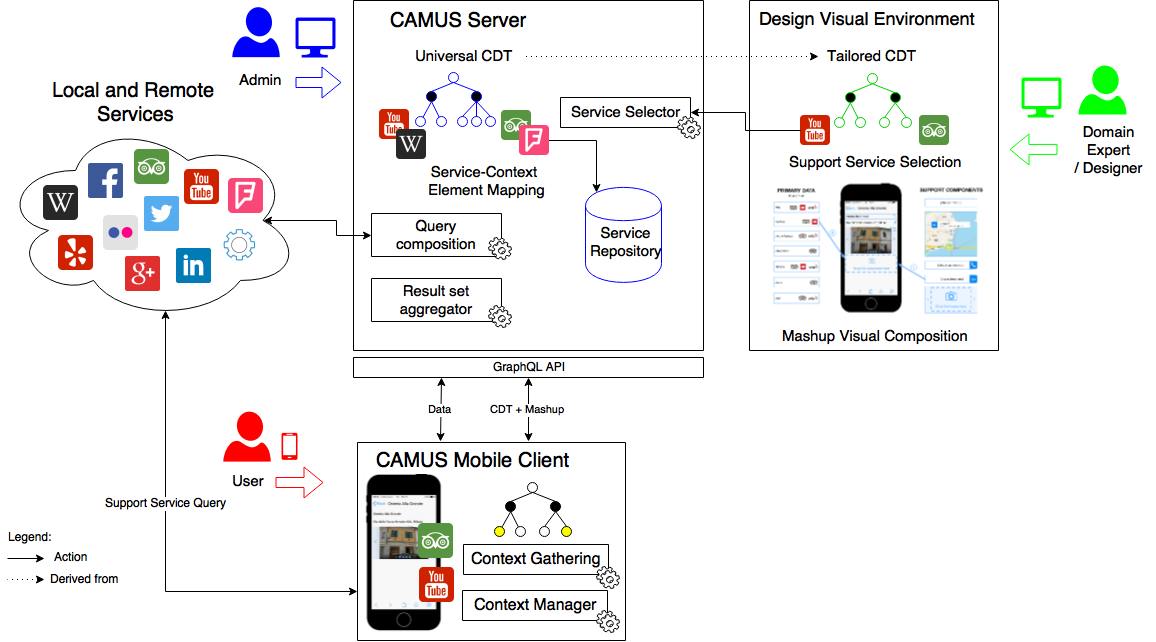
\includegraphics[width=\textwidth]{3-metodologia-camus/Immagini/architettura-generale.png}
	\caption{Architettura del sistema}\label{fig:architettura-sistema}
\end{figure}

Di seguito vengono elencati i tre componenti principali del sistema CAMUS:

\begin{enumerate}
	\item \textbf{Server}
	Il server è il punto in cui si interfaccia l'\emph{amministratore} di sistema ed è il punto dal quale è possibile avere una visione sulla complessità del sistema senza astrazioni. L'\emph{amministratore} ha i compiti di registrare i nuovi servizi e di configurare i termini per la trasformazione dei risultati ricevuti dai servizi. Inoltre definisce l'albero di contesto globale, che verrà utilizzato come base per la creazione di quelli personalizzati per gli utenti, e di associare le operazioni ai vari nodi che compongono l'albero
	\item \textbf{Web App}
	Le web app sono collegate all'\emph{esperto di settore} che compone l'applicazione mobile. Questo attore non è necessariamente un esperto di informatica e della tecnologia utilizzata, quindi ha bisogno di un astrazione maggiore rispetto all'amministratore. Sono disponibili due funzionalità di base: una permette di creare dei CDT personalizzati per gli utenti e di modificare le associazioni dei servizi, mentre l'altra permette di creare i mashup per le pagine dell'applicazione, collegando i termini con i componenti che verranno poi renderizzati in fase di esecuzione
	\item \textbf{App Mobile}
	La mobile app è l'interfaccia dell'\emph{utente} finale con il sistema. Essa ha il compito di renderizzare i mashup definiti dall'esperto e di permettere all'utente di specificare il proprio contesto per richiedere al server i risultati inerenti a esso. Oltre alle informazioni richieste all'utente vengono inoltre sfruttati i sensori messi a disposizione dal dispositivo (es.: coordinate geografiche, orario, ecc.) per migliorare la precisione del contesto, in modo trasparente all'utente.
	Una volta che l'utente finale ha effettuato l'accesso, vengono caricati gli schemi di mashup e l'albero di contesto specifico dell'utente. L'app si occuperà di renderizzare gli schemi ricevuti generando dinamicamente delle schermate che verranno utilizzate dall'utente per effettuare tutte le operazioni che desidera.
	I risultati vengono mostrati seguendo il pattern \emph{master-detail} \cite{molina2002user}: in prima istanza viene generato un elenco (\emph{master}) dei risultati ottenuti, mostrando poche informazioni riguardo il singolo elemento; successivamente l'utente può selezionare uno o più elementi della lista per visualizzare i dettagli (\emph{detail}) dell'elemento. In questa fase entrano in gioco i servizi di supporto: una volta che l'utente decide di visualizzare i dettagli di un elemento, l'app si occupa, in base allo schema di mashup corrente, di interrogare i servizi di supporto necessari per arricchire le informazioni che ha precedentemente ricevuto.
\end{enumerate}

\section{Modello del contesto\label{sec:modello-contesto}}

Come illustrato nella Sezione \ref{sec:context-awareness}, per il progetto CAMUS viene utilizzato il \emph{Context Dimension Tree} come modello per la rappresentazione del contesto. In questa sezione si vogliono mettere in evidenza le modifiche rese necessarie per adattare il modello alle esigenze del progetto. In particolare, oltre alla classificazione dei nodi originale del CDT, viene aggiunta un'ulteriore divisione in base al ruolo che un nodo può assumere durante la fase di selezione dei servizi:

\begin{itemize}
	\item \textbf{Nodo filtro}
	\upe la tipologia predefinita. I nodi di tipo filtro permettono, come si può dedurre dal nome, di filtrare i servizi che sono idonei all'utilizzo in un determinato contesto
	\item \textbf{Nodo ranking}
	Questa tipologia viene assegnata ad alcuni nodi specifici, come quello relativo alla \emph{località}, che assumono una maggiore importanza durante la selezione dei servizi, in quanto permettono di scegliere dei servizi che hanno un maggior impatto nel contesto specifico. Per esempio un nodo relativo alla \emph{località} permette di dare maggiore rilevanza ai servizi che sono più attinenti al luogo e che quindi forniscono delle informazioni più accurate
\end{itemize}

\section{Creazione dell'ecosistema dei servizi\label{sec:ecosistema-servizi}}

I servizi rappresentano un punto cardine del sistema, in quanto mettono a disposizione le risorse che verranno mostrate all'utente. Si è deciso di suddividerli in due categorie ben distinte, in base alla loro funzionalità:

\begin{enumerate}
	\item \textbf{Primari}
	Sono i servizi che vengono interrogati in prima istanza per acquisire le informazioni di interesse per il contesto nel quale si trova l'utente. Per esempio, se si effettua la ricerca di un ristorante, le informazioni principali saranno il nome del ristorante, l'indirizzo e il numero di telefono. TripAdvisor\footnote{TripAdvisor: \url{https://www.tripadvisor.it/}} e Zomato\footnote{Zomato: \url{https://www.zomato.com/it}} sono due esempi di servizi primari
	\item \textbf{Supporto}
	Sono i servizi che vengono utilizzati per arricchire le informazioni acquisite tramite i servizi primari. Possono mettere a disposizione dati aggiuntivi, contenuti multimediali (es.: foto e video) oppure possono fornire un'integrazione con altre app presenti sul dispositivo. Alcuni esempi di servizi di supporto sono quindi in grado di fornire informazioni sul meteo, la mappa del luogo o le indicazioni dei mezzi di trasporto per raggiungere il posto. Invece l'apertura del dialer telefonico quando viene selezionato il numero di telefono o l'utilizzo dell'app di navigazione preferita quando si sceglie un indirizzo rappresentano degli esempi di integrazione con altre app, che assumano pur sempre il ruolo di servizi di supporto anche se disponibile in locale sul dispositivo mobile dell'utente
\end{enumerate}

Per quanto queste categorie rappresentino una divisione molto precisa dei servizi, non vengono considerate come rigide. Come già evidenziato in \cite{rizzo2015progettazione}, ogni servizio espone una o più operazioni, e non è detto che tutte rientrino nella medesima categoria. Può capitare che un servizio metta a disposizione un'operazione che viene considerata primaria e un'altra che invece fornisce informazioni di supporto. Si è deciso quindi di non effettuare una categorizzazione a livello di servizio, bensì per ogni operazione, in modo da garantire una maggiore flessibilità.

Per coerenza, d'ora in avanti verrà utilizzata la nomenclatura \emph{operazione primaria} per riferirsi alle operazioni che forniscono le informazioni principali e \emph{operazione di supporto} per le operazioni che arricchiscono le informazioni primarie.

Per l'acquisizione dei dati è importante che il server sappia come interrogare i servizi e come interpretare le risposte. Si è deciso dunque di creare una repository composta dai \emph{descrittori dei servizi}, che contengono le informazioni necessarie per la gestione di tutti i servizi che possono essere utilizzati dal sistema. Ogni descrittore è composto da una prima parte relativa alle informazioni del servizio (es.: nome, categoria, url base, ecc.) e da una parte costituita dall'elenco delle operazioni che espone. La specifica delle operazioni fornisce le seguenti informazioni che permettono di effettuare le richieste:

\begin{itemize}
	\item \textbf{Elenco dei parametri}
	Per interrogare l'operazione di un servizio è necessario comporre una query con i dati che si vogliono richiedere. Queste informazioni sono dipendenti dalla specifica implementazione del servizio e variano tra diversi servizi. Nel descrittore vengono dunque elencati i parametri necessari per la composizione della query e dove andare a recuperare i relativi valori. L'acquisizione dei valori può avvenire secondo tre differenti modalità:
	\begin{enumerate}
		\item \emph{Default}
		Il valore viene impostato direttamente nel descrittore (es.: l'API key per l'autenticazione)
		\item \emph{Mapping CDT}
		Viene definita l'associazione con uno o più nodi del CDT e il valore viene recuperato in base alla selezione effettuata dall'utente (es.: le coordinate geografiche). Questi valori possono essere eventualmente trasformati da quelli simbolici del contesto a un'altra rappresentazione adatta per effettuare la query (es.: al valore \virgolette{Restaurant} del contesto viene associata la tipologia \virgolette{food})
		\item \emph{Mapping Term}
		Questa modalità viene utilizzata esclusivamente per i servizi di supporto e fornisce un placeholder nelle query che verrà rimpiazzato a runtime con il valore reale acquisito dalla risposta o dal dispositivo. Per esempio, se vogliamo ottenere l'indicazione del tempo necessario per raggiungere in bus il ristorante \virgolette{Vietnamonamour} dalla posizione corrente, l'url da interrogare assumerà la forma \textbf{http://www.example.com/\\maps/api/directions/json?origin=45.4789205,9.2343392\&\\destination=45.4815105,9.220423\&transit\_mode=bus}, dove in \emph{origin} vengono inserite le coordinate di dove si trova l'utente mentre in \emph{destination} vengono aggiunte le coordinate del ristorante da raggiungere. Quindi al parametro \emph{origin} vengono associati i \emph{termini} \virgolette{device\_latitude} e \virgolette{device\_longitude}, che corrispondono alle coordinate del dispositivo, mentre al parametro \emph{destination} vengono associati i termini \virgolette{latitude} e \virgolette{longitude}, che verranno recuperate a runtime dalla descrizione del ristorante. L'url che riceverà il dispositivo sarà simile alla seguente: \textbf{http://www.example.com/maps/api/directions/json?origin=\\\{device\_latitude\}, \{device\_longitude\}\&destination=\\\{latitude\},\{longitude\}\&transit\_mode=bus}
	\end{enumerate}
	\item \textbf{Schema della risposta}
	Per ottenere omogeneità tra le risposte ottenute dai diversi servizi, i dati ricevuti devono essere trasformati secondo uno schema comprensibile dalla mobile app. Per effettuare questa trasformazione vengono in aiuto i \emph{termini} (es.: titolo, indirizzo, descrizione, ecc.), che rappresentano le classi semantiche di appartenenza degli attributi. L'elenco dei termini disponibili viene mantenuto in una repository come per i descrittori dei servizi. Queste annotazioni hanno una duplice utilità: in primo luogo, definendo il significato semantico di ogni attributo, semplificano l'integrazione dei dati provenienti da diversi servizi, in secondo luogo semplificano la creazione dei mashup, come verrà approfonditamente trattato nella Sezione \ref{sec:mashup-design}, in quanto permettono di ragionare su categorie astratte di dati rispetto a dati reali forniti dai vari servizi e agevolano la riusabilità degli schemi in diversi contesti 
	\item \textbf{Gestione della paginazione}
	I dati che vengono restituiti a seguito di una query possono essere molteplici. Per semplificare la gestione delle risposte, i servizi implementano delle politiche di paginazione, dove vengono specificati il numero di risultati che si vogliono ottenere in una pagina e un numero che indica la pagina che è stata richiesta \cite{masse2011rest}. Questa sezione serve appositamente per indicare quali sono i parametri che vengono utilizzati dal servizio per richiamare le diverse pagine che compongono i risultati
\end{itemize}

\section{Associazione dei servizi al CDT\label{sec:associazione-servizi-cdt}}

Una volta che i servizi sono stati aggiunti alla repository è necessario specificare le associazioni che permettono la selezione dei servizi in base al contesto nel quale si trova l'utente.

Nel modello originale del CDT, presentato nella Sezione \ref{sec:context-dimension-model}, il processo di selezione dei dati rilevanti per un determinato contesto avveniva tramite la definizione di viste, che venivano create in linguaggio SQL e associate ai \emph{nodi valore}. Come evidenziato anche nella precedente ricerca \cite{rizzo2015progettazione}, questa metodologia non è più applicabile principalmente per due motivi:

\begin{enumerate}
	\item
	Si vuole rendere il funzionamento del sistema il più semplice possibile affinché possa essere utilizzato da persone che non hanno profonde conoscenze di informatica, la scrittura di query in SQL non è alla portata di chiunque
	\item
	Non avendo a disposizione direttamente i dati, bensì i servizi da invocare per acquisirli, la selezione tramite viste non è la più idonea a essere utilizzata
\end{enumerate}

Il nostro approccio prevede di associare le \emph{operazioni} ai \emph{nodi} dell'albero del contesto. In questo modo viene definita una strategia sì semplice ma allo stesso tempo funzionale, in quanto permette di definire con una buona libertà i contesti nei quali un'operazione ha senso di essere richiamata.

Queste associazioni vengono specificate unicamente sui nodi di tipo \emph{valore}, perché sono quelli che definiscono un contesto specifico. Non vengono invece imposti vincoli sul livello dei nodi verso i quali effettuare le associazioni. Generalmente le associazioni vengono definite nei nodi foglia ma, se un'operazione è valida per più di un contesto, può essere specificata in un nodo valore che ha uno o più figli. Per essere selezionata, un'operazione deve possedere almeno un'associazione con un nodo. Non viene invece imposto nessun limite superiore, in quanto un'operazione può essere associata a tanti nodi quanti sono i contesti nei quali è corretto che venga richiamata. Un'operazione non può essere aggiunta più volte all'interno di un nodo, in quanto è sufficiente una singola associazione affinché l'operazione venga presa in considerazione durante la fase di selezione.

Questo metodo è utile nella maggior parte dei casi per coprire le situazioni più comuni. In alcuni casi però è necessario prevedere dei meccanismi di selezione più complessi. Un esempio è dato dalle coordinate geografiche: quando si ha a che fare con un servizio locale è bene che venga associato nei dintorni di una specifica località, per due motivi in particolare: \emph{i)} all'esterno di quest'area non produrrebbe risultati; \emph{ii)} deve essere messo in risalto se l'utente si trova nel suo raggio d'azione, in quanto può fornire delle informazioni più accurate riguardo la zona. CAMUS prevede questo caso e in particolare è possibile associare un'operazione a una specifica latitudine e longitudine, che rappresentano solitamente il centro della città. Il sistema utilizza queste informazioni per definire una circonferenza, con centro dato dalle coordinate, e utilizza un raggio preimpostato al fine di selezionare tutti i servizi che rientrano nell'area definita.

Questo è solo un esempio di associazione particolare e potrebbero esisterne di ulteriori: il sistema è stato progetto in modo che sia estendibile tramite moduli sviluppati ad-hoc che possano gestire questi casi particolari. Ulteriori dettagli sull'implementazione vengono analizzati nella Sezione \ref{sec:primary-service-selection}.

Esistono delle distinzioni in base alla tipologia di operazione, se \emph{primaria} o di \emph{supporto}, in quanto cambia l'algoritmo di selezione.

Per quanto riguarda le \emph{operazioni primarie}, quando vengono associate a un determinato contesto viene definito anche un indice di \emph{priorità}: questo valore è un numero intero, a partire da 1 e crescente all'interno del singolo nodo, definisce l'importanza che il servizio assume in quel determinato contesto e verrà utilizzato nella fase di selezione dei servizi illustrata nella Sezione \ref{sec:selezione-operazioni}. Questo indicatore ha senso di essere utilizzato esclusivamente nei \emph{nodi valore}, in quanto contengono una raccolta generica di servizi, mentre per i \emph{nodi attributo} non è necessario, poiché l'ordinamento all'interno di una categoria di attributi non è sempre univoca. Se si prende per esempio un elenco di servizi associati a una città tramite le sue coordinate geografiche, si può considerare come indice di priorità la lontananza rispetto all'utente, che può essere calcolata solamente a runtime e può variare spesso.

Una menzione particolare viene riservata all'associazione con la dimensione \emph{Interest Topic}. Come precedentemente esposto nella Sezione \ref{sec:modello-contesto}, il modello del contesto deve essere in grado di adattarsi a diversi ambiti di utilizzo. Gli \emph{Interest Topic} fungono proprio da descrittori delle situazioni principali nelle quali l'utente può trovarsi. Un contesto specifico può essere molto complesso: gli \emph{Interest Topic} hanno il vantaggio di permettere la definizione di una categoria di riferimento, sulla quale poi specializzare la ricerca secondo le altre caratteristiche del contesto attive. Alcuni esempi di \emph{Interest Topic} sono i \virgolette{Ristoranti}, gli \virgolette{Hotel}, i \virgolette{Musei}, ecc.
Al fine di far rispettare questa classificazione è stato introdotto il vincolo che ogni \emph{operazione primaria} deve obbligatoriamente essere aggiunta ad almeno un \emph{Interest Topic}. Non viene imposto un vincolo sul numero di \emph{Interest Topic} differenti ai quali può essere associata un'operazione, in quanto può essere valida per ambiti differenti.

Per le \emph{operazioni di supporto} non è sempre necessario definire le associazioni con i nodi del CDT. Alcuni operazioni di supporto possono essere richiamate in modo statico quando non necessitano del contesto per essere scelte (es.: i servizi generici come Wikipedia\footnote{Wikipedia: \url{https://en.wikipedia.org/wiki/Main_Page}} o Flickr\footnote{Flickr: \url{https://www.flickr.com/}}). Per altre operazioni, come per esempio quelle relative ai mezzi di trasporto, è invece necessario basarsi sul contesto per selezionare la più idonea alla situazione. Per esempio, se un utente specifica che non dispone di un'auto e che si trova a Milano, allora il sistema proporrà i mezzi di trasporto pubblici presenti nella città, insieme all'elenco di altre tipologie di trasporto come i taxi o il car sharing. In questo caso è dunque necessario, come nel caso delle operazioni primarie, definire le associazioni delle operazioni con i nodi del CDT. Il processo di associazione è dunque simile a quello delle operazioni primarie, con la differenza che non bisogna specificare la priorità dei servizi.

\begin{figure}[ht]
	\centering
	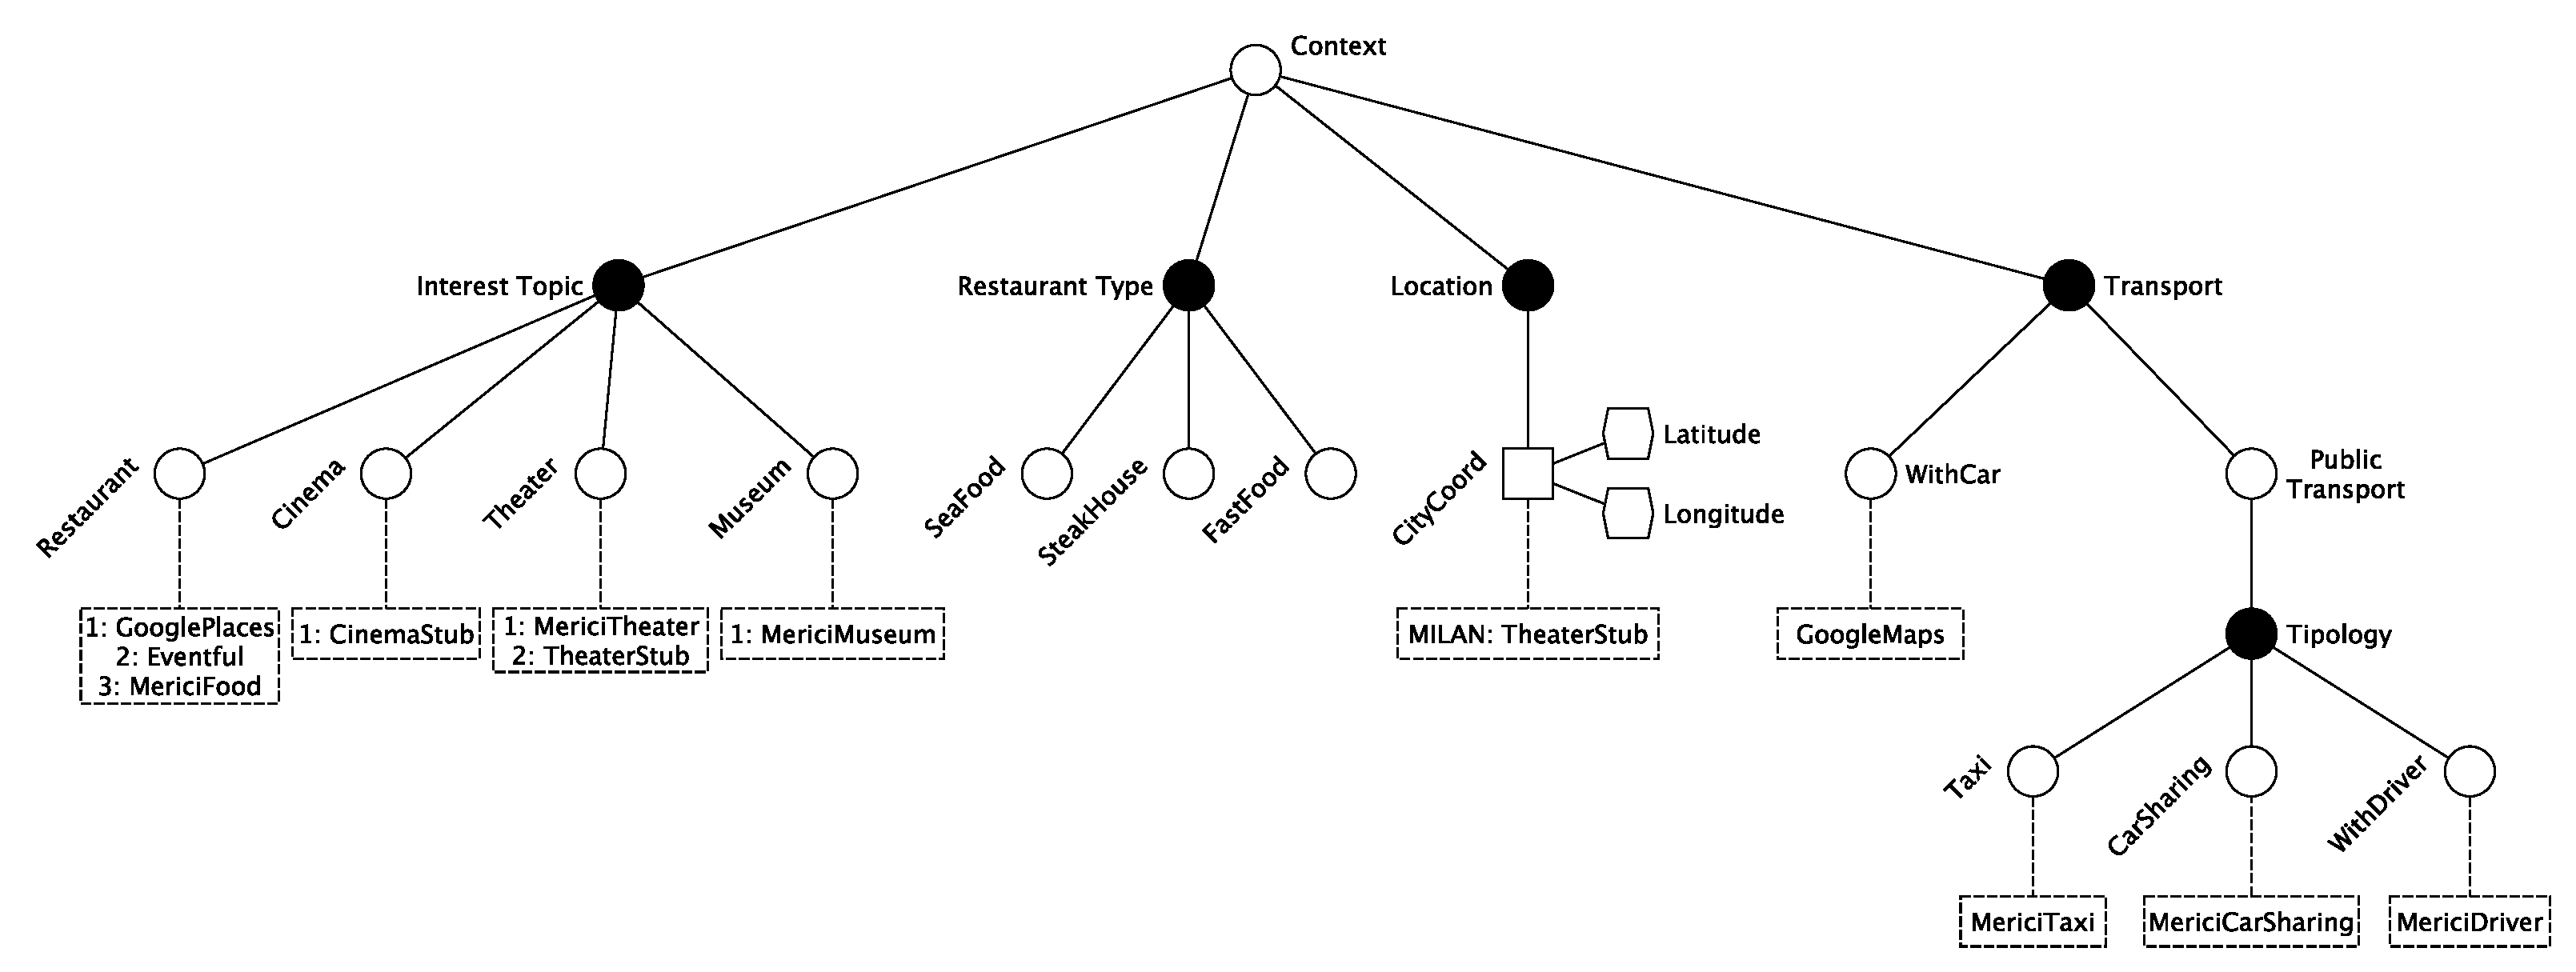
\includegraphics[width=\textwidth]{3-metodologia-camus/Immagini/associazioni-cdt.pdf}
	\caption{Associazione dei servizi al CDT}\label{fig:associazione-servizi-cdt}
\end{figure}

In Figura \ref{fig:associazione-servizi-cdt} viene mostrato un esempio di associazione. Viene rappresentato un contesto nel quale è possibile richiedere informazioni su \emph{ristoranti}, \emph{cinema}, \emph{teatri} e \emph{musei}. Sotto a ogni \emph{Interest Topic} vengono evidenziate, nei blocchi tratteggiati, le operazioni che sono associate allo specifico nodo. Si può notare che a ogni operazione viene assegnato un numero, che corrisponde alla \emph{priorità} che ha nella categoria.

Per i \emph{ristoranti} viene data anche la possibilità di scegliere la tipologia di cucina che si preferisce. A questi valori non vengono effettuate associazioni: infatti queste selezioni verranno utilizzate come parametro per i servizi.

Un'altra dimensione importante è la \emph{Località}, che definisce il punto nel quale si trova l'utente. Per rappresentare un posto vengono utilizzate le sue coordinate, che sono memorizzate nel parametro \emph{CityCoord}, il quale a sua volta viene specializzato nei campi \emph{Latitudine} e \emph{Longitudine}. In questo caso l'associazione dei servizi avviene definendo le coordinante del centro della città desiderata. Per semplificare l'immagine, è stato utilizzato il valore \virgolette{Milan}, per associare l'operazioni di ricerca dei teatri per Milano. In realtà andrebbero utilizzate le coordinate del centro città, che sono $ (45.46427, 9.18951) $.

Infine, con le dimensioni \emph{Trasporto} e \emph{Tipologia Trasporto} vengono definite le associazioni con le operazioni di supporto. La principale differenza con il caso delle operazioni primarie è che non viene definito nessun valore di priorità.

\section{CDT su misura per gli utenti\label{sec:cdt-su-misura}}

Il modello del CDT definito nella Sezione \ref{sec:associazione-servizi-cdt} viene chiamato \emph{CDT Universale}, in quanto rappresenta la rappresentazione del contesto più completo del quale il sistema dispone. Questo CDT deve descrivere tutti i possibili contesti che si vogliono gestire; possono coesistere diversi ambiti in parallelo, con le relative dimensioni che vanno a specializzare il dominio generale. Com'è facilmente intuibile, questo schema può diventare di enormi dimensioni, quindi inutilizzabile per via della moltitudine di selezioni possibili. Inoltre emerge il problema dei \emph{contesti non validi}, cioè quei contesti che non possono esistere nella realtà. Per esempio, scegliere come \emph{Interest Topic} la ricerca di \virgolette{Ristoranti} e selezionare di voler fare un viaggio \virgolette{Rilassante} non è un contesto valido, in quanto la dimensione \virgolette{Tipologia di Viaggio} ha senso di essere attivata solo quando viene selezionato come \emph{Interest Topic} quello relativo ai viaggi. Queste due problematiche vanno in senso contrario con i principi di usabilità e semplicità che sono stati presi come linee guida per il progetto.

Una prima soluzione consiste nell'introdurre l'elenco delle \emph{dimensioni consentite} per ogni \emph{Interest Topic}. In questo modo, nella fase di scelta delle dimensioni che si vogliono attivare, l'interfaccia grafica può essere aggiornata in seguito a ogni selezione, mostrando solamente le dimensioni che è possibile scegliere senza generare conflitti. In questo modo si risolverebbero entrambi i problemi sopra citati, in quanto l'elenco delle \emph{dimensioni consentite} permette di ridurre il numero totale di contesti generabili e impedisce la selezione di dimensioni che porterebbero a effettuare delle selezioni erronee.

Per quanto questa soluzione sia tecnicamente valida, rimane aperta un'ulteriore questione: all'utente potrebbero venire proposte comunque una serie di opzioni che non sono di suo interesse. Per esempio, un utente deve pianificare un viaggio e non possiede animali e nel CDT viene definita una dimensione \virgolette{Con Animali Domestici}, per specificare che bisogna cercare strutture che ammettano l'accesso anche agli animali. In questa situazione verrebbe ogni volta proposta la selezione del possesso animali all'utente, mentre potrebbe essere sempre omessa in quanto non utile nella descrizione del contesto di quello specifico utente.

Per risolvere questa ulteriore problematica, relativa più al profilo specifico di ogni utente, si è pensato di far entrare in gioco la figura dell'\emph{esperto di settore}: l'esperto è la persona alla quale si deve rivolgere l'utente per ottenere una personalizzazione dell'app. Come verrà descritto nella sezione \ref{sec:mashup-design}, l'esperto di settore è colui che ha il compito di adattare l'aspetto della mobile app, andando a  modificare lo schema di mashup. Si è deciso dunque che si tratta della figura più indicata anche per adattare il contesto al profilo specifico di ogni utente. Nasce quindi l'idea di creare dei CDT specifici per gli utenti, che mostrano solamente le dimensioni che sono di loro interesse. Questi CDT vengono definiti come \emph{CDT su misura} o \emph{Tailored CDT}. In pratica, all'esperto di settore viene dato in carico il compito di \emph{eliminare} le dimensioni che non sono utili all'utente e che creerebbero solamente confusione. Questi alberi di contesto vengono creati a partire dallo schema globale e modificati dall'\emph{esperto di settore} appositamente per uno specifico utente. Oltre alla possibilità di eliminare le dimensioni del contesto non necessarie, viene data anche la libertà di effettuare ulteriori modifiche per migliorare l'esperienza dell'utente:

\begin{itemize}
	\item
	Viene data la possibilità di impostare dei valori predefiniti. Questa caratteristica è sempre correlata con il profilo dell'utente e da un certo punto di vista è un problema simile a quello esposto in precedenza riguardo le dimensioni non interessanti. In questo caso però, invece che rimuovere totalmente un ramo dell'albero, viene assegnato un valore che rimane sempre valido. Questa caratteristica è molto importante, ed è utile che coesista insieme alla possibilità di rimuovere le dimensioni non interessanti. Si prenda per esempio un utente che non dispone di un proprio mezzo di trasporto: in questo caso non si può rimuovere completamente la dimensione che riguarda i \emph{Trasporti}, in quanto all'utente può sempre interessare come muoversi con i mezzi pubblici. \upe invece più conveniente fissare il valore \virgolette{Trasporto Pubblico} per segnalare che l'utente utilizzerà sempre i mezzi di trasporto pubblici per raggiungere i luoghi di suo interesse, in modo che la app generata permetta soltanto di sceglierne la tipologia, e non scegliere il trasporto con mezzi propri
	\item
	\upe possibile inoltre modificare le associazioni delle operazioni con i nodi del CDT, comprese, solo per le \emph{operazioni primarie}, le priorità che assumono all'interno di ogni nodo. Questa funzionalità tende a sfruttare in maniera più marcata le conoscenze dell'\emph{esperto di settore} per migliorare la qualità dei risultati ottenuti dal sistema. Può essere utilizzata per diversi scopi, come favorire l'uso di determinati servizi rispetto ad altri o sostituirne alcuni che in una certa località non sono disponibili o non forniscono dei buoni risultati.
\end{itemize}

\section{Selezione delle operazioni in base al contesto\label{sec:selezione-operazioni}}

Nelle precedenti sezioni è stato spiegato come è possibile aggiungere nuovi servizi nel sistema, come vengono associati al contesto e infine come è possibile personalizzare il contesto in base alle preferenze dei singoli utenti.

Resta da definire il metodo col quale a runtime questi servizi vengono selezionati. Questa fase è una tra le più importanti all'interno di CAMUS, in quanto la selezione dei servizi da utilizzare impatta in maniera preponderante sulla qualità e rilevanza dei dati che verranno mostrati all'utente. \upe necessario quindi definire un algoritmo che tenga conto della situazione nella quale si trova l'utente e, a partire da questa, selezioni le operazioni più idonee a soddisfare la richiesta. 

Si ricorda che un \emph{contesto} è formato dalla congiunzione tra uno o più elementi del contesto, che a loro volta sono formati dalla \emph{dimensione} di riferimento e dal \emph{valore} o \emph{parametri} che essa assume. In Figura \ref{fig:esempio-contesto} viene mostrato un esempio di contesto in cui si vogliono cercare i ristoranti con cucina a base di pesce nei dintorni di Lambrate.

\begin{figure}[ht]
	\begin{align*}
	C =\ &InterestTopic : Restaurant\ \land \\
	&RestaurantType : SeaFood\ \land \\
	&Transport : PublicTransport\ \land \\
	&Location\ (Latitude : ``45.478897" \land Longitude : ``9.2342429")
	\end{align*}
	\caption{Esempio di contesto\label{fig:esempio-contesto}}
\end{figure}

Un contesto può essere dunque visto come un elenco di coppie {<}dimensione, valore{>}, che rappresentano i nodi selezionati dall'utente. La ricerca delle associazioni che hanno validità nelle singole coppie avviene tramite una ricerca \emph{chiave-valore}, dove la \emph{chiave} è l'etichetta della dimensione mentre il \emph{valore} è il valore specifico assunto dalla dimensione, tra le associazioni definite nell'albero di contesto.

Questo metodo non è sempre utilizzabile: come già introdotto nella Sezione \ref{sec:associazione-servizi-cdt} esistono alcune associazioni particolari che necessitano di apposite funzioni per essere ricercate. L'elenco generato da queste funzioni viene integrato con quello prodotto dalla ricerca tramite $ {<}dimensione, valore{>} $.

Una menzione particolare va fatta al caso dei nodi \emph{contesto} che hanno dei figli. Visto che la maggior parte delle associazioni viene definita sui nodi foglia, selezionare un nodo che non sia foglia porterebbe a non trovare nessuna associazione. Lo pseudocodice utilizzato per la selezione dei nodi figlio viene presentato nell'Algoritmo \ref{alg:algoritmo-ricerca-nodi-figlio}. L'idea è che se un utente seleziona un nodo a un livello superiore significa che è indifferente rispetto alle sue specializzazioni, che dunque devono essere a loro volta considerate.

\begin{algorithm}
	\caption{Algoritmo di ricerca dei nodi figlio}
	\label{alg:algoritmo-ricerca-nodi-figlio}
	\begin{algorithmic}
		\Require
		\Statex $cdt$ \Comment The decorated CDT
		\Statex $nodes$ \Comment The list of active nodes
		\Ensure
		\Statex $childList$ \Comment List of child nodes found
		\Statex
		\State $nodeValues \gets nodes.map('value')$ \Comment Acquire list of values selected
		\ForAll {$ item\; in\; cdt.context $}
		\State $ intersection \gets intersect(item.parents, nodeValues) $
		\If {$ !isEmpty(interesection) $}
		\ForAll {$ value\; in\; item.values $}
		\State $ childList.push(\{ $
		\State\hspace{\algorithmicindent} $ name: item.name, $
		\State\hspace{\algorithmicindent} $ value: value $
		\State $ \}) $
		\EndFor
		\EndIf
		\EndFor\\
		\Return $ childList $
	\end{algorithmic}
\end{algorithm}

Ogni nodo ha associato l'elenco di nodi dai quali discende, a partire dalla radice. Viene controllato nell'albero del contesto se esistono dei nodi che hanno nel loro elenco dei parenti uno dei nodi che sono stati scelti dall'utente. Ogni nodo che soddisfa questa regola viene a sua volta selezionato.

\begin{figure}[ht]
	\centering
	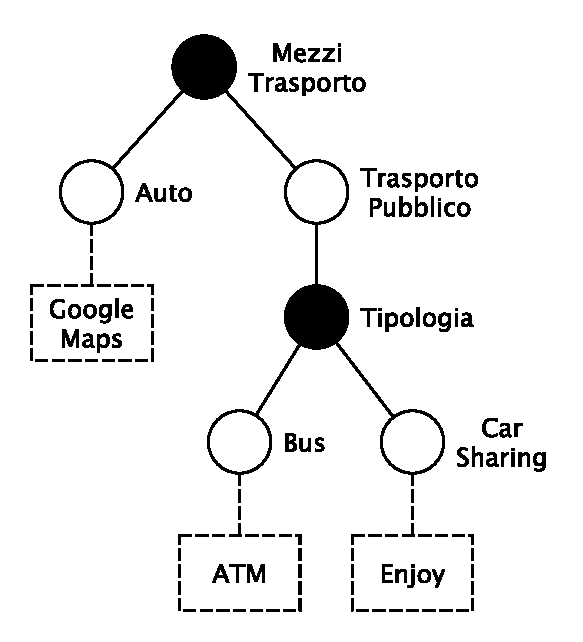
\includegraphics[width=0.4\textwidth]{3-metodologia-camus/Immagini/esempio-gerarchia.pdf}
	\caption{Esempio gerarchia}\label{fig:esempio-gerarchia}
\end{figure}

In Figura \ref{fig:esempio-gerarchia} viene mostrato un esempio di albero gerarchico. Nel caso in cui l'utente scelga un qualsiasi nodo foglia la selezione avviene come nei casi esposti. Invece per il contesto $ C = MezziTrasporto: TrasportoPubblico $ deve essere trattato separatamente, in quanto il valore \emph{Trasporto Pubblico} possiede un nodo figlio. In questo caso la selezione del valore \emph{Trasporto Pubblico} significa che per l'utente è indifferente prendere una tipologia di mezzo piuttosto che un'altra. Il problema che emerge riguarda le associazioni con le operazioni: come si può notare nell'esempio, le operazioni vengono associate solamente ai nodi foglia. Quindi il contesto precedente porterebbe alla selezione di nessuna operazione. Per risolvere questo problema viene definito che, quando viene selezionato un nodo che ha dei figli, tutti i suoi discendenti vengono automaticamente selezionati. In definitiva, il precedente contesto diventa $ C' = MezziTrasporto: TrasportoPubblico\ \land\ Tipologia: Bus\ \land\ Tipologia: Taxi $.

Come già evidenziato nella Sezione \ref{sec:associazione-servizi-cdt}, le associazioni vengono effettuate seguendo due approcci differenti in base alla tipologia dell'operazione, \emph{primaria} oppure di \emph{supporto}. Il motivo principale risiede nel fatto che queste tipologie di operazione hanno scopi differenti e necessitano dunque di due approcci di selezione appositi. Di seguito vengono analizzati entrambi i metodi utilizzati in CAMUS, concentrandosi su di una tipologia di operazione alla volta. Si parte dal presupposto che sia già stata eseguita la ricerca delle associazioni esposta in precedenza.

\subsection*{Operazioni primarie}

Come esposto nella Sezione \ref{sec:associazione-servizi-cdt}, ogni operazione viene associata a uno o più nodi dell'albero di contesto e a ognuna di queste associazioni viene assegnato un valore che rappresenta la \emph{priorità} che l'operazione assume all'interno del nodo. Il primo passo per la selezione delle operazioni è l'assegnazione di un \emph{punteggio} a ogni operazione che ha una o più corrispondenze all'interno dell'albero di contesto. 

La ricerca delle associazioni fornisce come risultato un elenco delle operazioni che sono adatte all'utilizzo nello specifico contesto, assieme al relativo valore di priorità, per ogni associazione trovata. \upe necessario introdurre un ulteriore parametro che influisce nella formula per l'assegnamento del \emph{punteggio} alle operazioni: il \emph{peso} dei nodi. Come definito nella Sezione \ref{sec:modello-contesto}, vengono introdotte due nuove tipologie di nodo: \emph{filtro} e \emph{ranking}. Le associazioni trovate tramite funzioni personalizzate vengono sempre intese come nodi di tipo \emph{ranking}. Il \emph{peso} di un nodo viene assegnato in base alla \emph{tipologia} del nodo, rispettando il vincolo:

\begin{equation*}
w_{FILTRO} < w_{RANKING} \quad \forall\ n \in CDT
\end{equation*}

In pratica, a ogni nodo \emph{filtro} deve essere assegnato un peso strettamente minore rispetto a un nodo \emph{ranking}. Il punteggio \emph{R} di ogni operazione \emph{o} viene calcolato tramite la funzione:

\begin{equation}\label{eq:primary-service-formula}
R_o = \sum_{i \in SA(o)}{\frac{w_i}{p_i}}
\end{equation}

dove \emph{SA(o)} rappresenta l'insieme dei nodi associati all'operazione \emph{o}, $ w_i $ e $ p_i $ rappresentano rispettivamente il \emph{peso} e il valore di \emph{priorità} dell \emph{i}-esimo nodo. Una volta calcolati i \emph{punteggi}, l'elenco delle operazioni viene riordinato in modo \emph{decrescente} e vengono selezionati le top-N operazioni. In Figura \ref{fig:esempio-punteggio-primari} viene definito un contesto di esempio con le associazioni delle operazioni primarie ai vari nodi dell'albero.

\begin{figure}[ht]
	\centering
	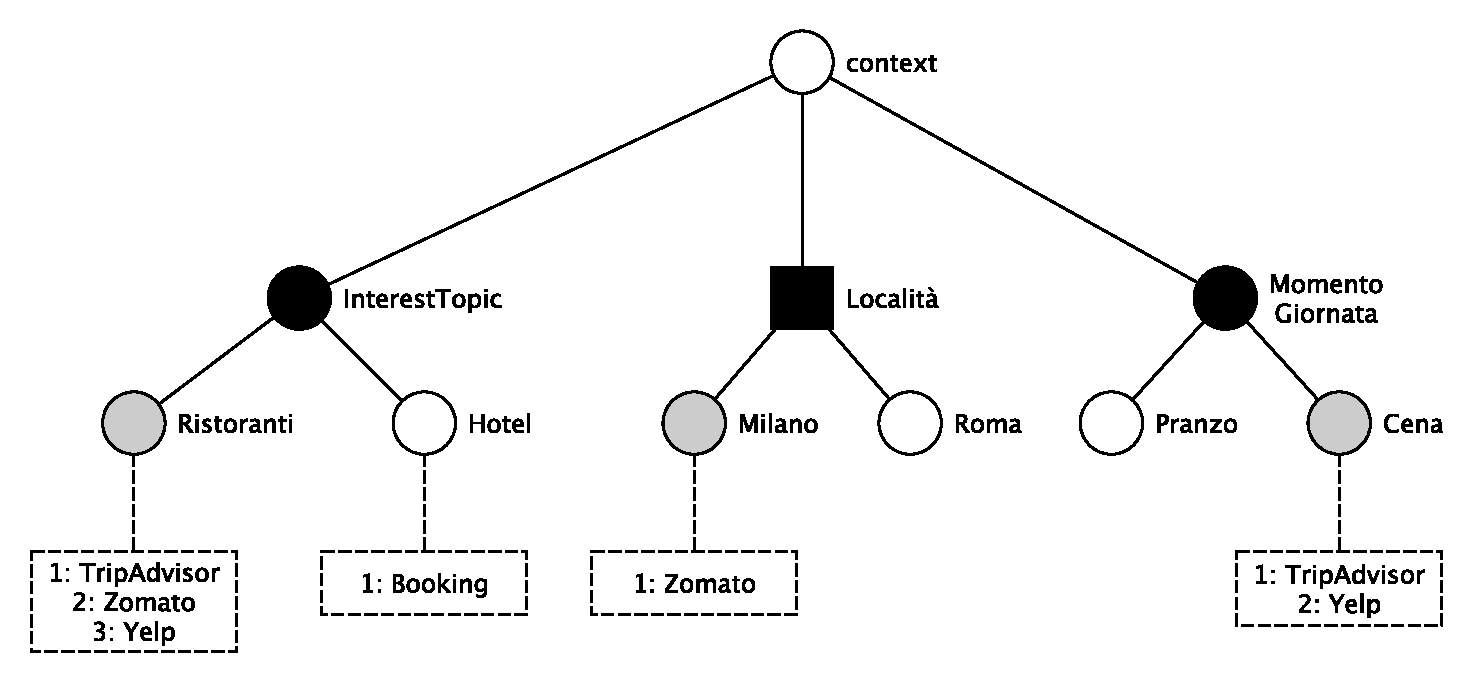
\includegraphics[width=\textwidth]{3-metodologia-camus/Immagini/esempio-punteggio-primari.pdf}
	\caption{Esempio di assegnazione del punteggio per le operazioni primarie}\label{fig:esempio-punteggio-primari}
\end{figure}

I nodi \emph{Interest Topic} e \emph{Momento Giornata} sono di tipo \emph{filtro} mentre il nodo \emph{Località} è di tipo \emph{ranking} (come evidenziato dalla diversa forma utilizzata). I nodi foglia di colore grigio sono quelli selezionati, che corrispondono al contesto $ C = InterestTopic: Ristoranti\ \land\ Localit\acute{a}: Milano\ \land\ MomentoGiornata: Cena $. Dalla fase di ricerca vengono selezionate le operazioni dei servizi $ \{TripAdvisor, Zomato,\\ Yelp\} $. Considerando come pesi dei nodi $ w_{FILTER} = 1 $  e $ w_{RANKING} = 4 $, viene calcolato il punteggio per ogni operazione:

\begin{align*}
R_{TripAdvisor} &= \frac{1}{1} + \frac{1}{1} = 2 \\
R_{Zomato} &= \frac{1}{2} + \frac{4}{1} = \frac{9}{2} = 4,5\\
R_{Yelp} &= \frac{1}{3} + \frac{1}{2} = \frac{5}{6} \approx 0,83
\end{align*} 

Riordinando la lista si ottiene $ \{ Zomato, TripAdvisor, Yelp \} $ e scegliendo i top-2 risultati si ottiene la selezione finale $ \{ Zomato, TripAdvisor \} $.

\subsection*{Operazioni di supporto}

A differenza delle operazioni primarie, per quelle di supporto non viene definito un valore di \emph{priorità}. Quindi la precedente funzione per il calcolo del punteggio non è applicabile. \upe stata inoltre considerata un'ulteriore problematica per la quale la precedente funzione non è utilizzabile. Per esempio, si consideri un servizio di supporto che fornisce indicazioni sui mezzi di trasporto pubblici. Molti di questi servizi hanno validità locale, infatti ogni città ha il proprio gestore per il servizio di trasporto pubblico (es. ATM\footnote{ATM: \url{www.atm.it}} per Milano e ATAC\footnote{ATAC: \url{www.atac.it}} per Roma). Quindi, nella fase di calcolo del punteggio, anche questi servizi verrebbero considerati e in alcune situazioni erroneamente selezionati come risultato finale. Si è optato per un metodo di selezione più rigido rispetto al caso delle operazioni primarie. In questo caso la ricerca delle associazioni produce un elenco di operazioni senza altri dati annessi. Di questa lista viene successivamente effettuato il \emph{conteggio} del numero di associazioni totali per ogni operazione. A ogni operazione viene inoltre conservato il \emph{numero minimo di associazioni} che devono essere rispettate. Vengono selezionate solamente le operazioni che rispettano le seguenti regole:

\begin{enumerate}
	\item
	le operazioni hanno un conteggio pari al numero minimo di associazioni e il valore del conteggio è pari al valore massimo trovato tra tutte le associazioni
	\item
	se il primo filtro non ha prodotto risultati, vengono selezionate le operazioni che hanno un conteggio superiore al numero minimo di associazioni, restituite in ordine decrescente secondo il valore del conteggio
\end{enumerate}

In questo modo vengono definite due regole, la prima più restrittiva mentre la seconda, che viene applicata solamente nel caso la prima non produca risultati, permette di avere un grado di libertà maggiore.

La prima regola permette di ottenere risultati che rispettano esattamente il numero minimo di associazioni imposto. Preferendo le operazioni con il valore più alto del conteggio permette la selezione delle operazioni che sono maggiormente conformi al contesto corrente.

Nel caso questa ricerca non sia soddisfatta entra in gioco la seconda regola. In questo caso viene semplicemente imposto che il valore del conteggio sia maggiore rispetto al numero minimo di associazioni. L'elenco delle operazioni viene ordinato in modo decrescente sempre in base al valore del conteggio, per mettere in risalto, come nel caso precedente, le operazioni più attinenti al contesto.

L'introduzione di questa seconda regola nasce dall'esigenza dettata dal fatto che un'operazione può essere associata a più di un nodo dell'albero. Questa affermazione viene chiarita meglio dal seguente esempio. Si ipotizzi che un'operazione sia associata a due nodi, entrambi figli dello stesso padre. Inoltre questo nodo padre discenda da un altro nodo. A questa operazione verrà dunque assegnato un numero minimo di associazioni pari a uno, perché è sufficiente che uno dei due nodi sia selezionato affinché l'operazione possa essere scelta. Tuttavia l'utente può selezionare anche il nodo dal quale il padre discende e anche in questo caso l'operazione può essere selezionata. Questa selezione porterebbe invece a un conteggio pari a due e quindi la prima regola scarterebbe l'operazione in quanto non ha il valore del conteggio pari al numero minimo di associazioni. Il secondo vincolo permette di gestire correttamente anche questa evenienza.

In Figura \ref{fig:esempio-selezione-supporto} viene mostrato un contesto di esempio con le associazioni delle operazioni di supporto ai vari nodi dell'albero.

\begin{figure}[ht]
	\centering
	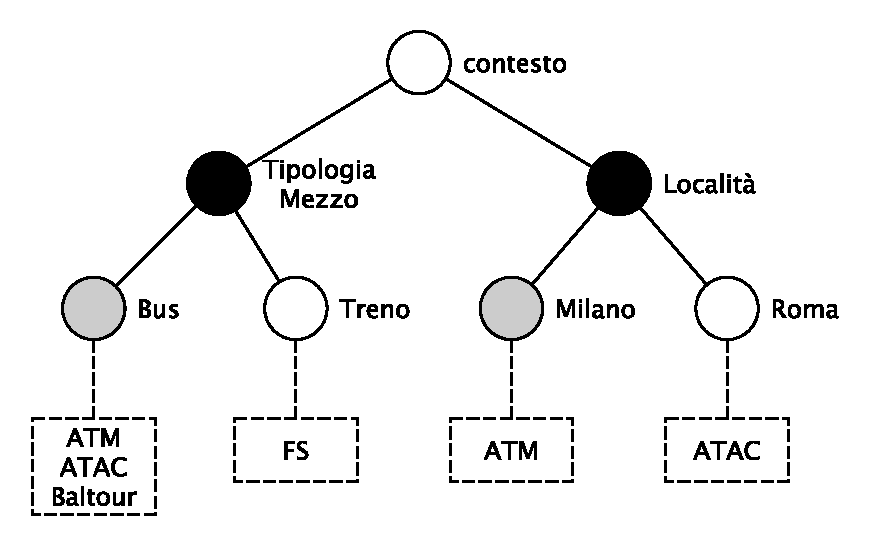
\includegraphics[width=0.5\textwidth]{3-metodologia-camus/Immagini/esempio-selezione-supporto.pdf}
	\caption{Esempio di selezione delle operazioni di supporto}\label{fig:esempio-selezione-supporto}
\end{figure}

I nodi attivi sono evidenziati in grigio ed equivalgono al contesto $ C = Tipologia\\Mezzo: Bus\ \land\ Localit\acute{a}: Milano $. Per le operazioni \emph{ATM} e \emph{ATAC} vengono definite due associazioni, mentre per le operazioni \emph{FS\footnote{Ferrovie dello Stato: \url{http://www.trenitalia.com/}}} e \emph{Baltour\footnote{Tour operator di bus su tutta Italia: \url{www.baltour.it}}} viene effettuata una singola associazione. La fase di ricerca restituisce le operazioni \emph{ATM} con conteggio pari a due e le operazioni \emph{ATAC} e \emph{Baltour} entrambe con conteggio pari a uno. Le operazioni che hanno un valore del conteggio pari al numero minimo di associazioni sono \emph{ATM} e \emph{Baltour}. Alla fine verrà selezionata solamente l'operazione relativa al servizio \emph{ATM}, in quanto possiede il valore massimo del conteggio. Come si può notare, quest'ultimo filtro permette di selezionare le operazioni che hanno una maggiore rilevanza per il contesto corrente, escludendo le operazioni che forniscono risultati meno precisi.

\section{Integrazione dei dati\label{sec:integrazione-dati}}

Una volta selezionati i servizi che più si adattano al contesto dell'utente, il passo successivo è interrogarli per acquisire le risposte. Dopo che sono state ricevute le informazioni si presenta un nuovo problema: ogni servizio ha il proprio formato di risposta. \upe necessario dunque fare sì che tutte le risposte vengano trasformate in una rappresentazione comune tale che sia utilizzabile dall'app mobile. Al fine di effettuare questa trasformazione vengono utilizzati una serie di \emph{termini semantici}: questi termini permettono di identificare univocamente una risorsa all'interno delle varie rappresentazioni ricevute, associando a ogni attributo il rispettivo valore semantico. Come precedentemente introdotto nella Sezione \ref{sec:ecosistema-servizi}, le associazioni tra gli elementi di una risposta e il termine di riferimento viene definito nel descrittore del servizio. In seguito alla trasformazione viene creato un set di risposte unificato, composto da tutti i dati ricevuti dai servizi.

Un ulteriore problema che si è dovuto affrontare riguarda gli elementi duplicati: può accadere che due o più servizi restituiscano dati relativi a una stessa entità. Questi dati duplicati devono essere unificati a formare una singola istanza. Il termine \virgolette{fondere} viene usato di proposito, in quanto anche gli elementi duplicati possono essere utilizzati per arricchire le informazioni ottenute. Si prenda per esempio due servizi che restituiscono il medesimo ristorante: il primo fornisce informazioni sul \emph{nome} del ristorante, l'\emph{indirizzo} e il \emph{numero di telefono} mentre il secondo mette a disposizione sempre il \emph{nome}, l'\emph{indirizzo}, l'\emph{url} del sito web e l'\emph{indirizzo email}. Come si può notare non è conveniente semplicemente ignorare uno dei due risultati in quanto si perderebbero alcuni informazioni che possono essere rilevanti. La procedura che viene adottata in questi casi è quella appunto di \emph{fondere} i due elementi. Resta da definire come comportarsi nel caso dei dati in comune tra gli elementi. Nell'esempio precedente si tratta del \emph{nome} del ristorante e del suo \emph{indirizzo}. In questa situazione entra in gioco il \emph{punteggio} del servizio calcolato come descritto nella Sezione \ref{sec:selezione-operazioni}. Vengono mantenute solamente le informazioni in comune fornite dal servizio col punteggio più elevato. Questa scelta ha una semplice spiegazione: si ipotizza che il servizio col punteggio migliore fornisca i dati più affidabili rispetto a un altro servizio con un punteggio inferiore.

L'altro punto importante nella ricerca degli elementi duplicati riguarda il numero di confronti da eseguire. Infatti, per effettuare un'analisi approfondita sarebbe necessario analizzare tutte le possibili coppie di elementi, che equivale a un algoritmo con complessità temporale $ O(n^2) $. Tuttavia alcuni confronti potrebbero essere evitati. Per esempio, se due ristoranti hanno un nome completamente diverso, è ovvio che non possono essere duplicati.

Come mostrato dallo pseudocodice dell'Algoritmo \ref{alg:algoritmo-rimozione-duplicati}, per evitare i confronti inutili il dataset viene diviso in vari \virgolette{bucket}. All'interno di questi \emph{bucket} vengono inseriti gli elementi che hanno una certa somiglianza tra loro. Questa tecnica viene chiamata \emph{blocking} \cite{elmagarmid2007duplicate} e permette di migliorare l'efficienza dell'algoritmo, in quanto si occupa di raggruppare l'intero dataset in porzioni ridotte in base alla somiglianza degli elementi che ne fanno parte. Per assegnare ogni elemento a uno specifico \emph{bucket} viene utilizzato l'algoritmo denominato \virgolette{Soundex} \cite{odell1918soundex}. Questo algoritmo genera un codice per ogni elemento in base alla pronuncia fonetica. Questo codice viene utilizzato come \emph{chiave} per l'assegnazione dell'elemento a uno specifico \emph{bucket}. Per effettuare questa operazione viene utilizzato per il confronto esclusivamente il campo \virgolette{titolo} dell'elemento.

Una volta che i \emph{bucket} sono stati creati, è necessario effettuare una comparazione più approfondita all'interno dei singoli gruppi, in quanto l'appartenenza allo stesso gruppo indica che esiste una certa affinità tra gli elementi ma non garantisce che siano duplicati. Vengono dunque effettuate delle comparazioni tra ogni coppia di elementi appartenenti allo stesso \emph{bucket}. Questa comparazione produce come risultato un valore di similarità. Se questo valore è superiore a una soglia predefinita, allora gli elementi sono duplicati. Per calcolare l'indice di somiglianza viene utilizzato il coefficiente di Dice \cite{dice1945measures}. In questo caso vengono presi in considerazione tutti i campi che sono in comune tra gli elementi in analisi. Ogni volta che due elementi risultano come duplicati vengono \emph{fusi} tramite la tecnica descritta precedentemente.

\begin{algorithm}
	\caption{Algoritmo di rimozione dei duplicati}
	\label{alg:algoritmo-rimozione-duplicati}
	\begin{algorithmic}
		\Require
		\Statex $ response $ \Comment The list of items received
		\Ensure
		\Statex $ output $ \Comment The results list without duplicates
		\Statex
		\ForAll{$ item\; in\; responses $}
		\State $ class\_key \gets Soundex(item.title) $
		\State $ buckets.add(class\_key, item) $
		\EndFor
		\ForAll{$ items\; in\; buckets $}
		\State $ len \gets items.length $
		\If{$ len > 1 $}
		\State $ i \gets 0 $
		\While{$ i < len $}
		\State $ j \gets i + 1 $
		\While{$ j < len $}
		\State $ sim\_value \gets calculateObjectSimilarity(items[i], items[j])$
		\If{$ sim\_value > threshold $}
		\If{$ items[i].rank \ge items[j].rank $}
		\State $ items[i] \gets mergeItems(items[i], items[j]) $
		\State $ items.remove(j) $
		\Else
		\State $ items[j] \gets mergeItems(items[j], items[i]) $
		\State $ items.remove(i) $
		\EndIf
		\State $ len \gets len - 1 $
		\Else
		\State $ j \gets j + 1 $
		\EndIf
		\EndWhile
		\State $ output.push(items[i]) $
		\State $ i \gets i + 1 $
		\EndWhile
		\Else
		\State $ output.push(items[0]) $
		\EndIf
		\EndFor\\
		\Return $ output $
	\end{algorithmic}
\end{algorithm}

Analizzando la struttura di questo algoritmo risulta però che la complessità temporale resta sempre pari a $ O(n^2) $, in quanto se tutti gli elementi hanno il medesimo codice fonetico verrebbero aggiunti in un singolo bucket, costringendo a eseguire tutti i confronti. Questa situazione è un caso molto raro: si assume che gli elementi vengano distribuiti in modo uniforme all'interno dei bucket. In genere i bucket saranno composti al massimo da un numero di elementi pari al numero di servizi interrogati. Infatti generalmente gli elementi duplicati appartengono a servizi diversi. Questo valore può variare leggermente in alcuni casi particolari. Può capitare per esempio che elementi distinti tra loro possano essere aggiunti allo stesso bucket a causa della loro pronuncia fonetica simile. Nel caso medio si ottiene che questo algoritmo abbia una complessità $ \Omega(nm^2) $, dove \emph{n} rappresenta il numero di elementi e \emph{m} la lunghezza massima di un bucket, con $ m \lll n $. In Figura \ref{fig:tempo-esecuzione-algoritmo-duplicati} è stato effettuato un confronto tra la versione \virgolette{vecchia} dell'algoritmo, dove venivano effettuati tutti i confronti, e quella \virgolette{nuova}, con le ottimizzazioni attive. \upe stato utilizzato un dataset composto dall'elenco dei ristoranti di Milano proveniente da quattro diversi servizi e con un elevato numero di elementi simili ($ 81\% $). Come si può notare il nuovo algoritmo ha un incremento lineare dei tempi di esecuzione all'aumentare del numero di elementi, come ci si poteva aspettare.

\begin{figure}[ht]
	\centering
	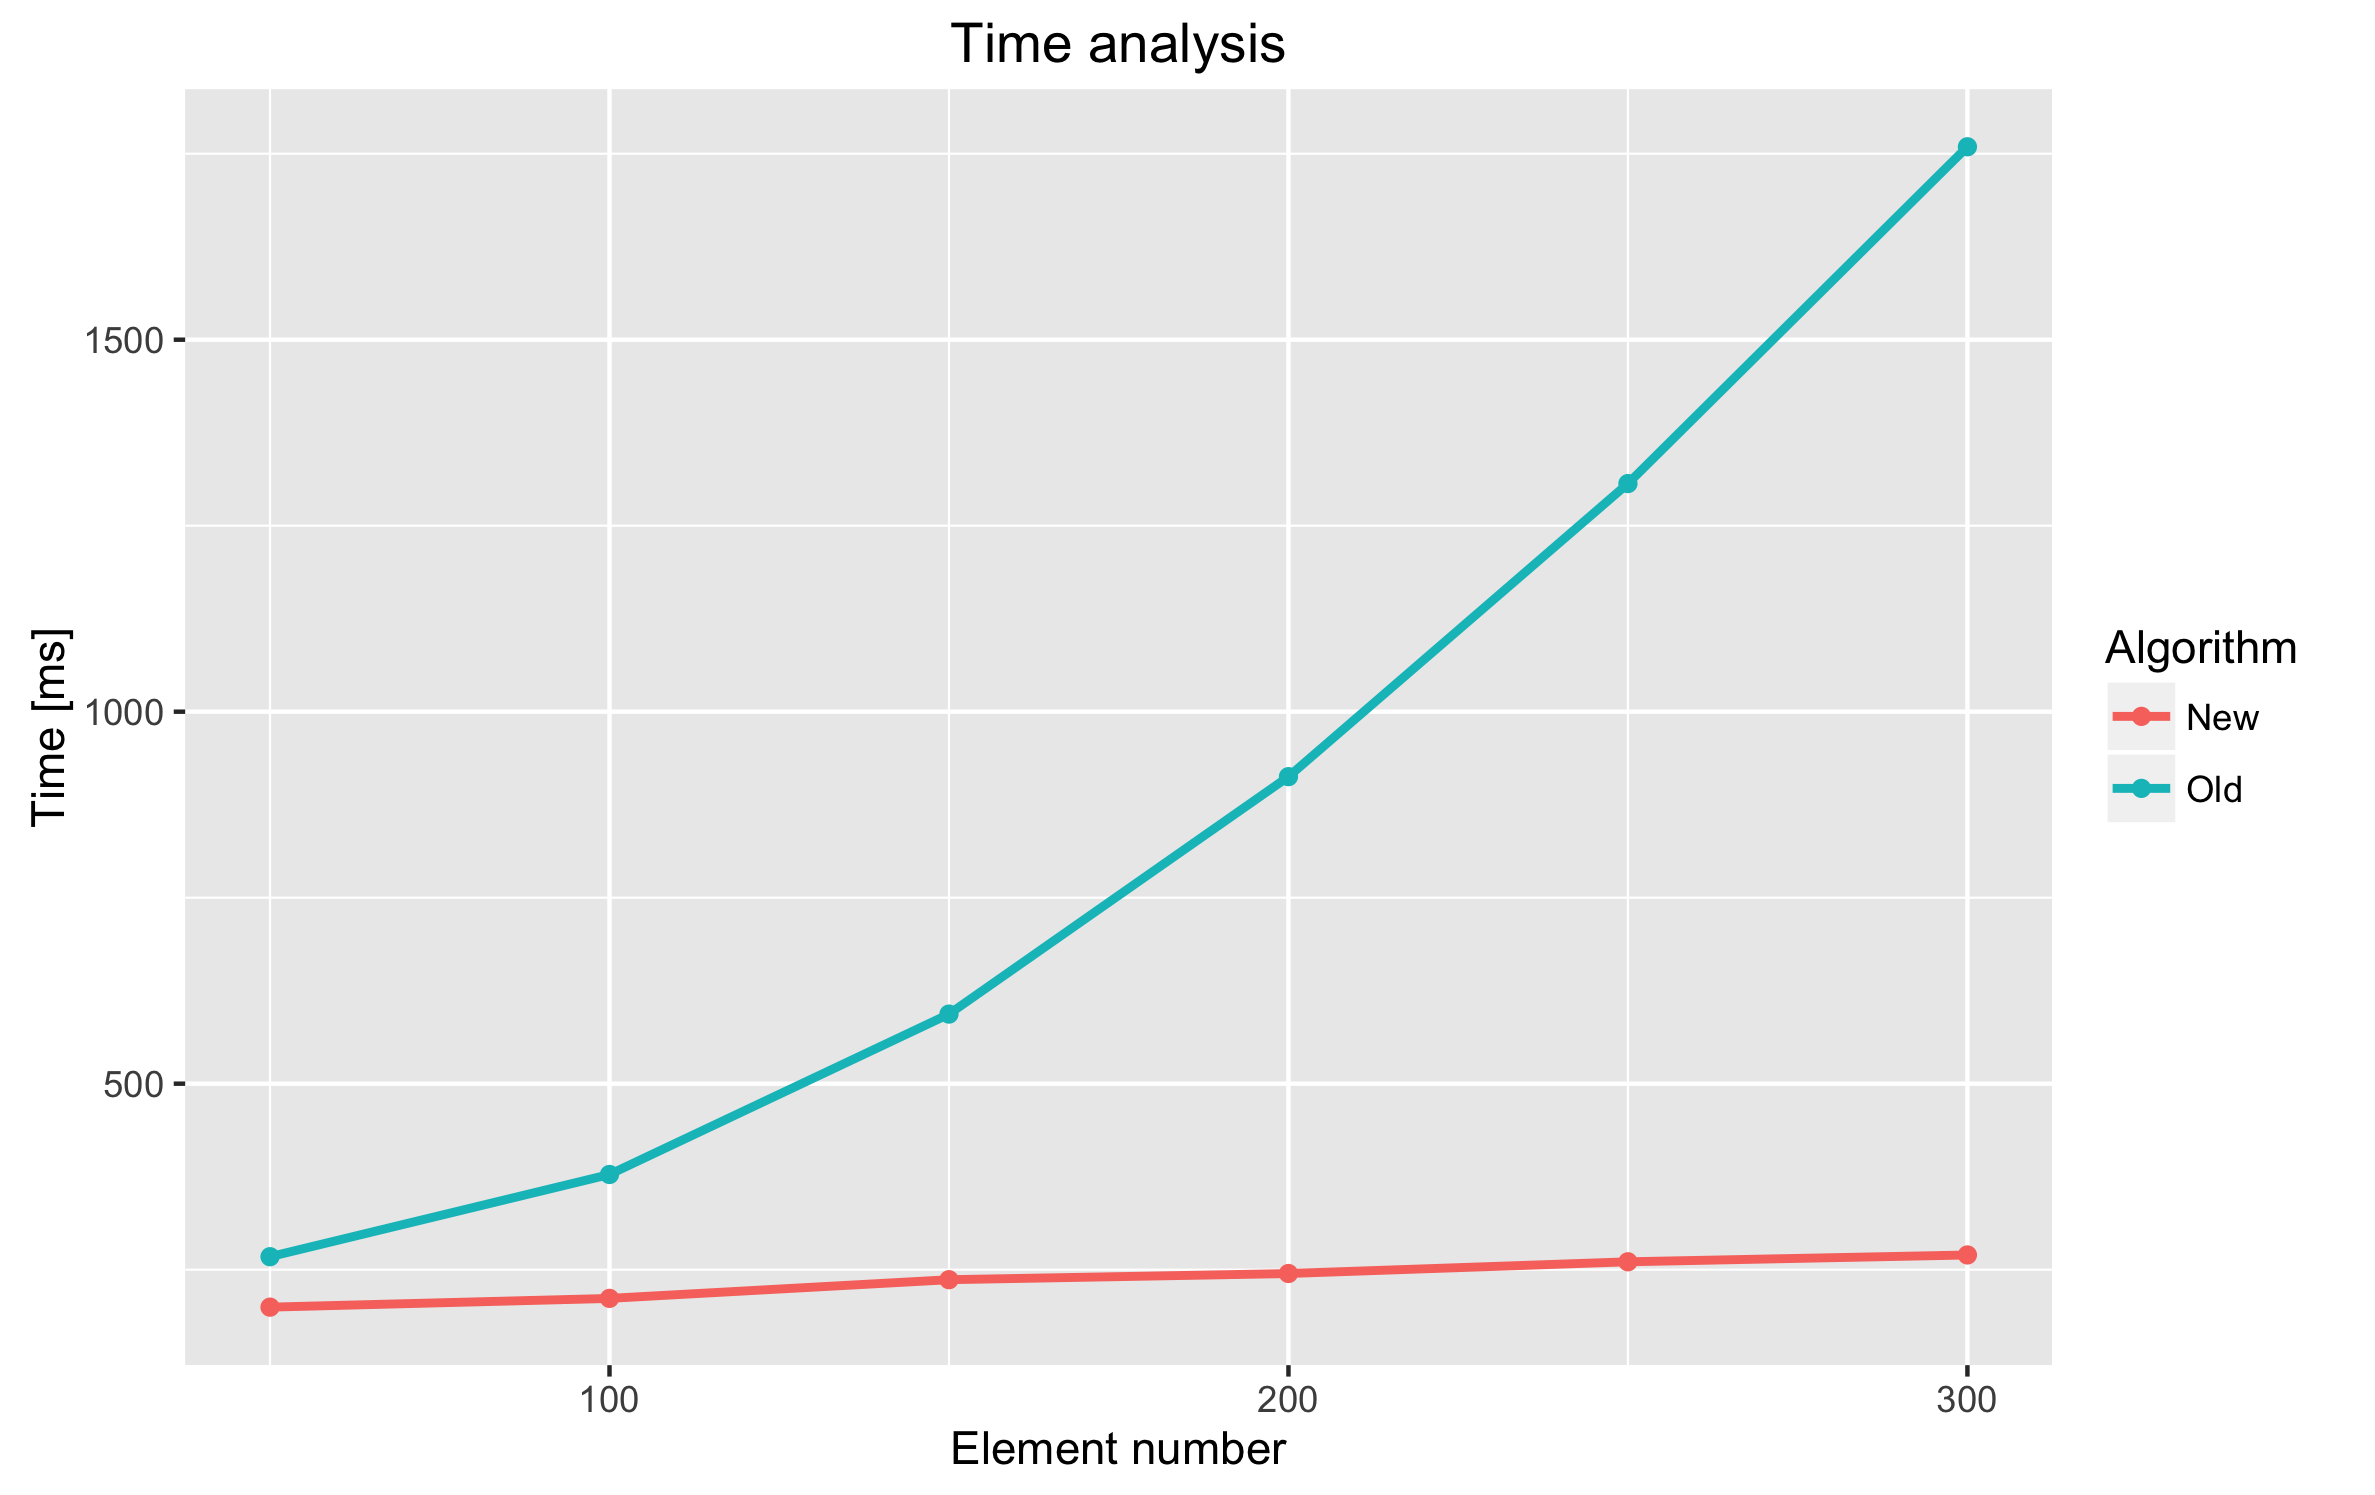
\includegraphics[width=\textwidth]{3-metodologia-camus/Immagini/similarity_time_analysis.png}
	\caption{Tempi di esecuzione algoritmo di ricerca duplicati}\label{fig:tempo-esecuzione-algoritmo-duplicati}
\end{figure}

Si è andati a effettuare anche un'analisi delle prestazioni dell'algoritmo. A partire da un dataset composto da 100 ristoranti, acquisito da 4 differenti servizi e composto per l'$ 81\% $ da elementi duplicati, si è verificato quali di questi elementi vengono correttamente etichettati come duplicati. Per valutare la bontà dell'algoritmo sono stati utilizzati i seguenti indicatori:

\begin{itemize}
	\item \textbf{Precision} Rappresenta la proporzione di documenti pertinenti fra quelli recuperati
	\item \textbf{Recall} Rappresenta il rapporto di documenti pertinenti che sono stati correttamente recuperati. Viene definita come la proporzione fra il numero di documenti rilevanti recuperati e il numero di tutti i documenti rilevanti disponibili nella collezione considerata
\end{itemize}

Queste due misure permettono di fornire un'indicazione su come si comporta l'algoritmo. Per calcolarle vengono utilizzate le seguenti formule:

\begin{center}
	\begin{minipage}[t]{0.5\textwidth}
		\begin{equation*}
		Precision = \frac{TP}{TP + FP}
		\end{equation*}
	\end{minipage}%
	\begin{minipage}[t]{0.5\textwidth}
		\begin{equation*}
		Recall = \frac{TP}{TP + FN}
		\end{equation*}
	\end{minipage}
\end{center}

Dove \emph{TP} significa \virgolette{True Positive}, \emph{FP} sta per \virgolette{False Positive} e \emph{FN} per \virgolette{False Negative}. In Tabella \ref{table:confusion-matrix} viene chiarito il significato di questi parametri.

\begin{table}[ht]
	\caption{Confusion Matrix}
	\label{table:confusion-matrix}
	\begin{tabularx}{\textwidth}{l | cc}
		\toprule
		& \textbf{Predetto Positivo} & \textbf{Predetto Negativo} \\
		\midrule
		\textbf{Condizione Positiva} & True Positive & False Negative  \\
		\hline
		\textbf{Condizione Negativa} & False Positive & True Negative \\
		\bottomrule
	\end{tabularx}
\end{table}

Per il caso in analisi i \emph{True Positive} sono gli elementi correttamente identificati come duplicati, i \emph{False Positive} sono gli elementi che sono stati identificati come duplicati ma non lo sono e \emph{False Negative} sono gli elementi duplicati che non sono stati rilevati. L'unico parametro configurabile dell'algoritmo è il \emph{threshold}, cioè la soglia minima affinché due elementi vengano identificati come duplicati. In Figura \ref{fig:prestazioni-algoritmo-duplicati} vengono mostrati i risultati ottenuti.

\begin{figure}[ht]
	\centering
	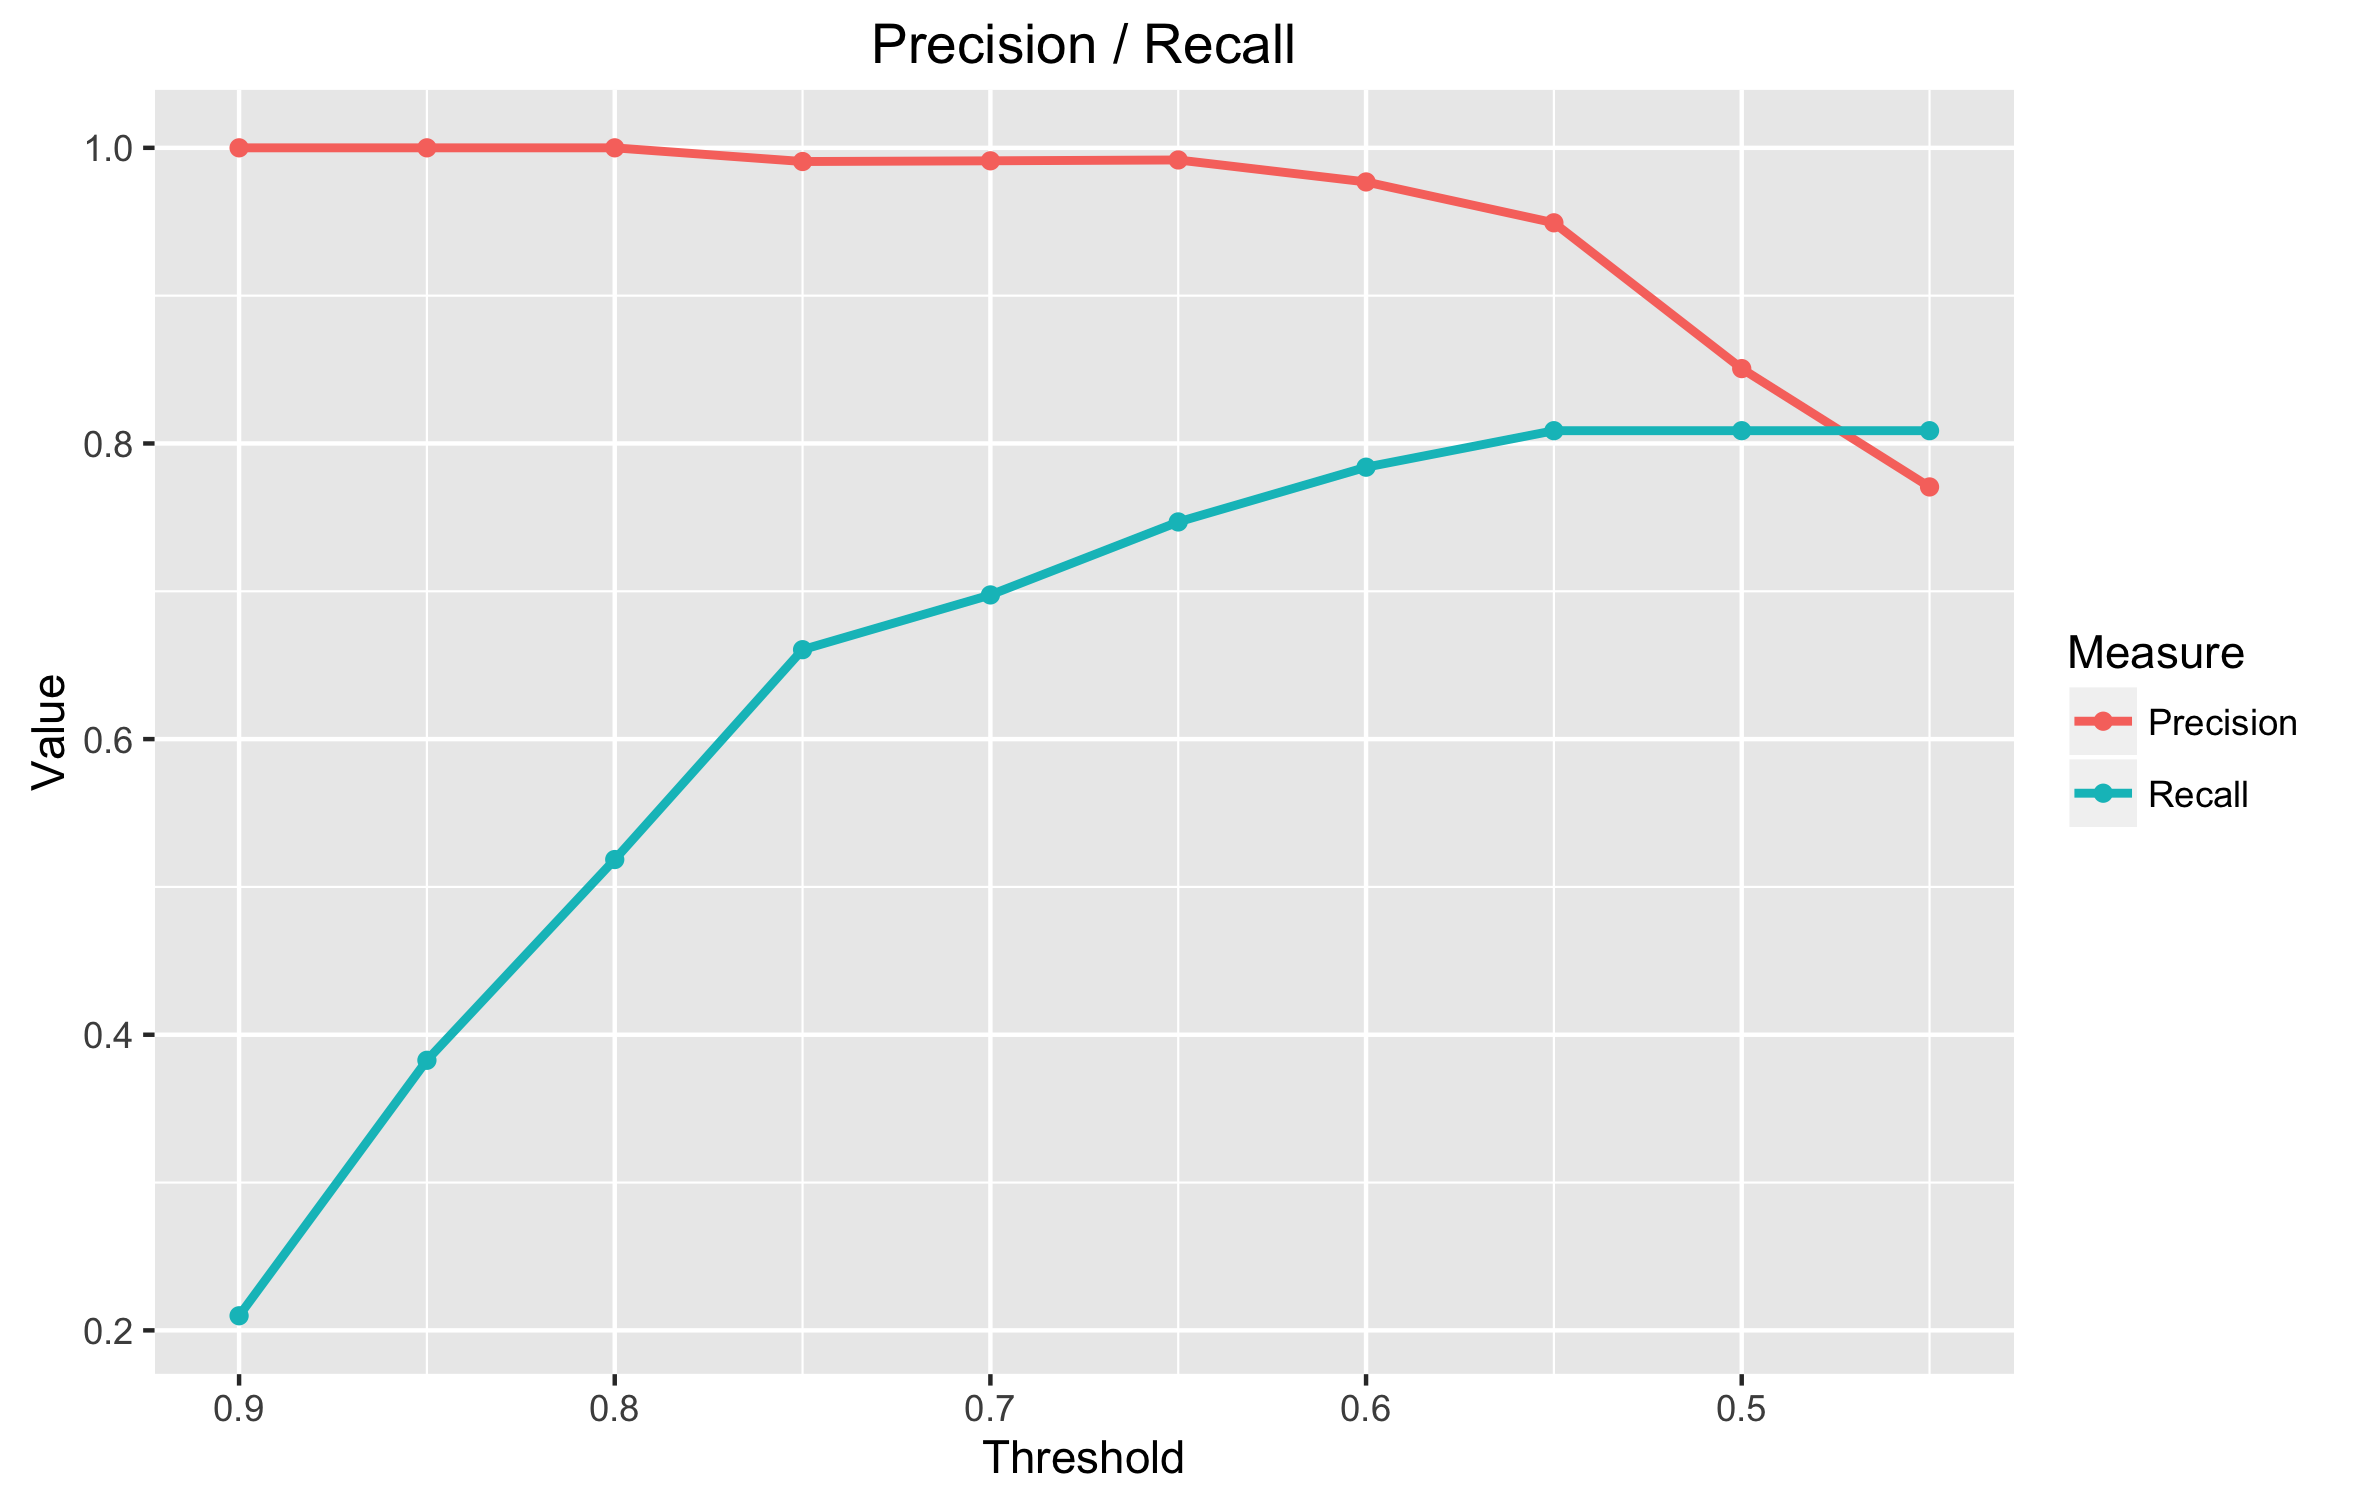
\includegraphics[width=\textwidth]{3-metodologia-camus/Immagini/similarity_precision_recall.png}
	\caption{Prestazioni dell'algoritmo di ricerca dei duplicati}\label{fig:prestazioni-algoritmo-duplicati}
\end{figure}

Alti valori del \emph{threshold} permettono di avere una \emph{precision} del $ 100\% $, il che significa che non sono presenti falsi positivi. Il contro è avere un valore di \emph{recall} molto basso: in pratica molti elementi duplicati non vengono identificati. Calibrare il valore di \emph{threshold} è un compito delicato: bisogna cercare di bilanciare l'esigenza di trovare il maggior numero di duplicati possibili con quella di non sbagliare le rilevazioni con elementi che sono estranei.

\section{Mashup Design\label{sec:mashup-design}}

\begin{figure}[ht]
	\centering
	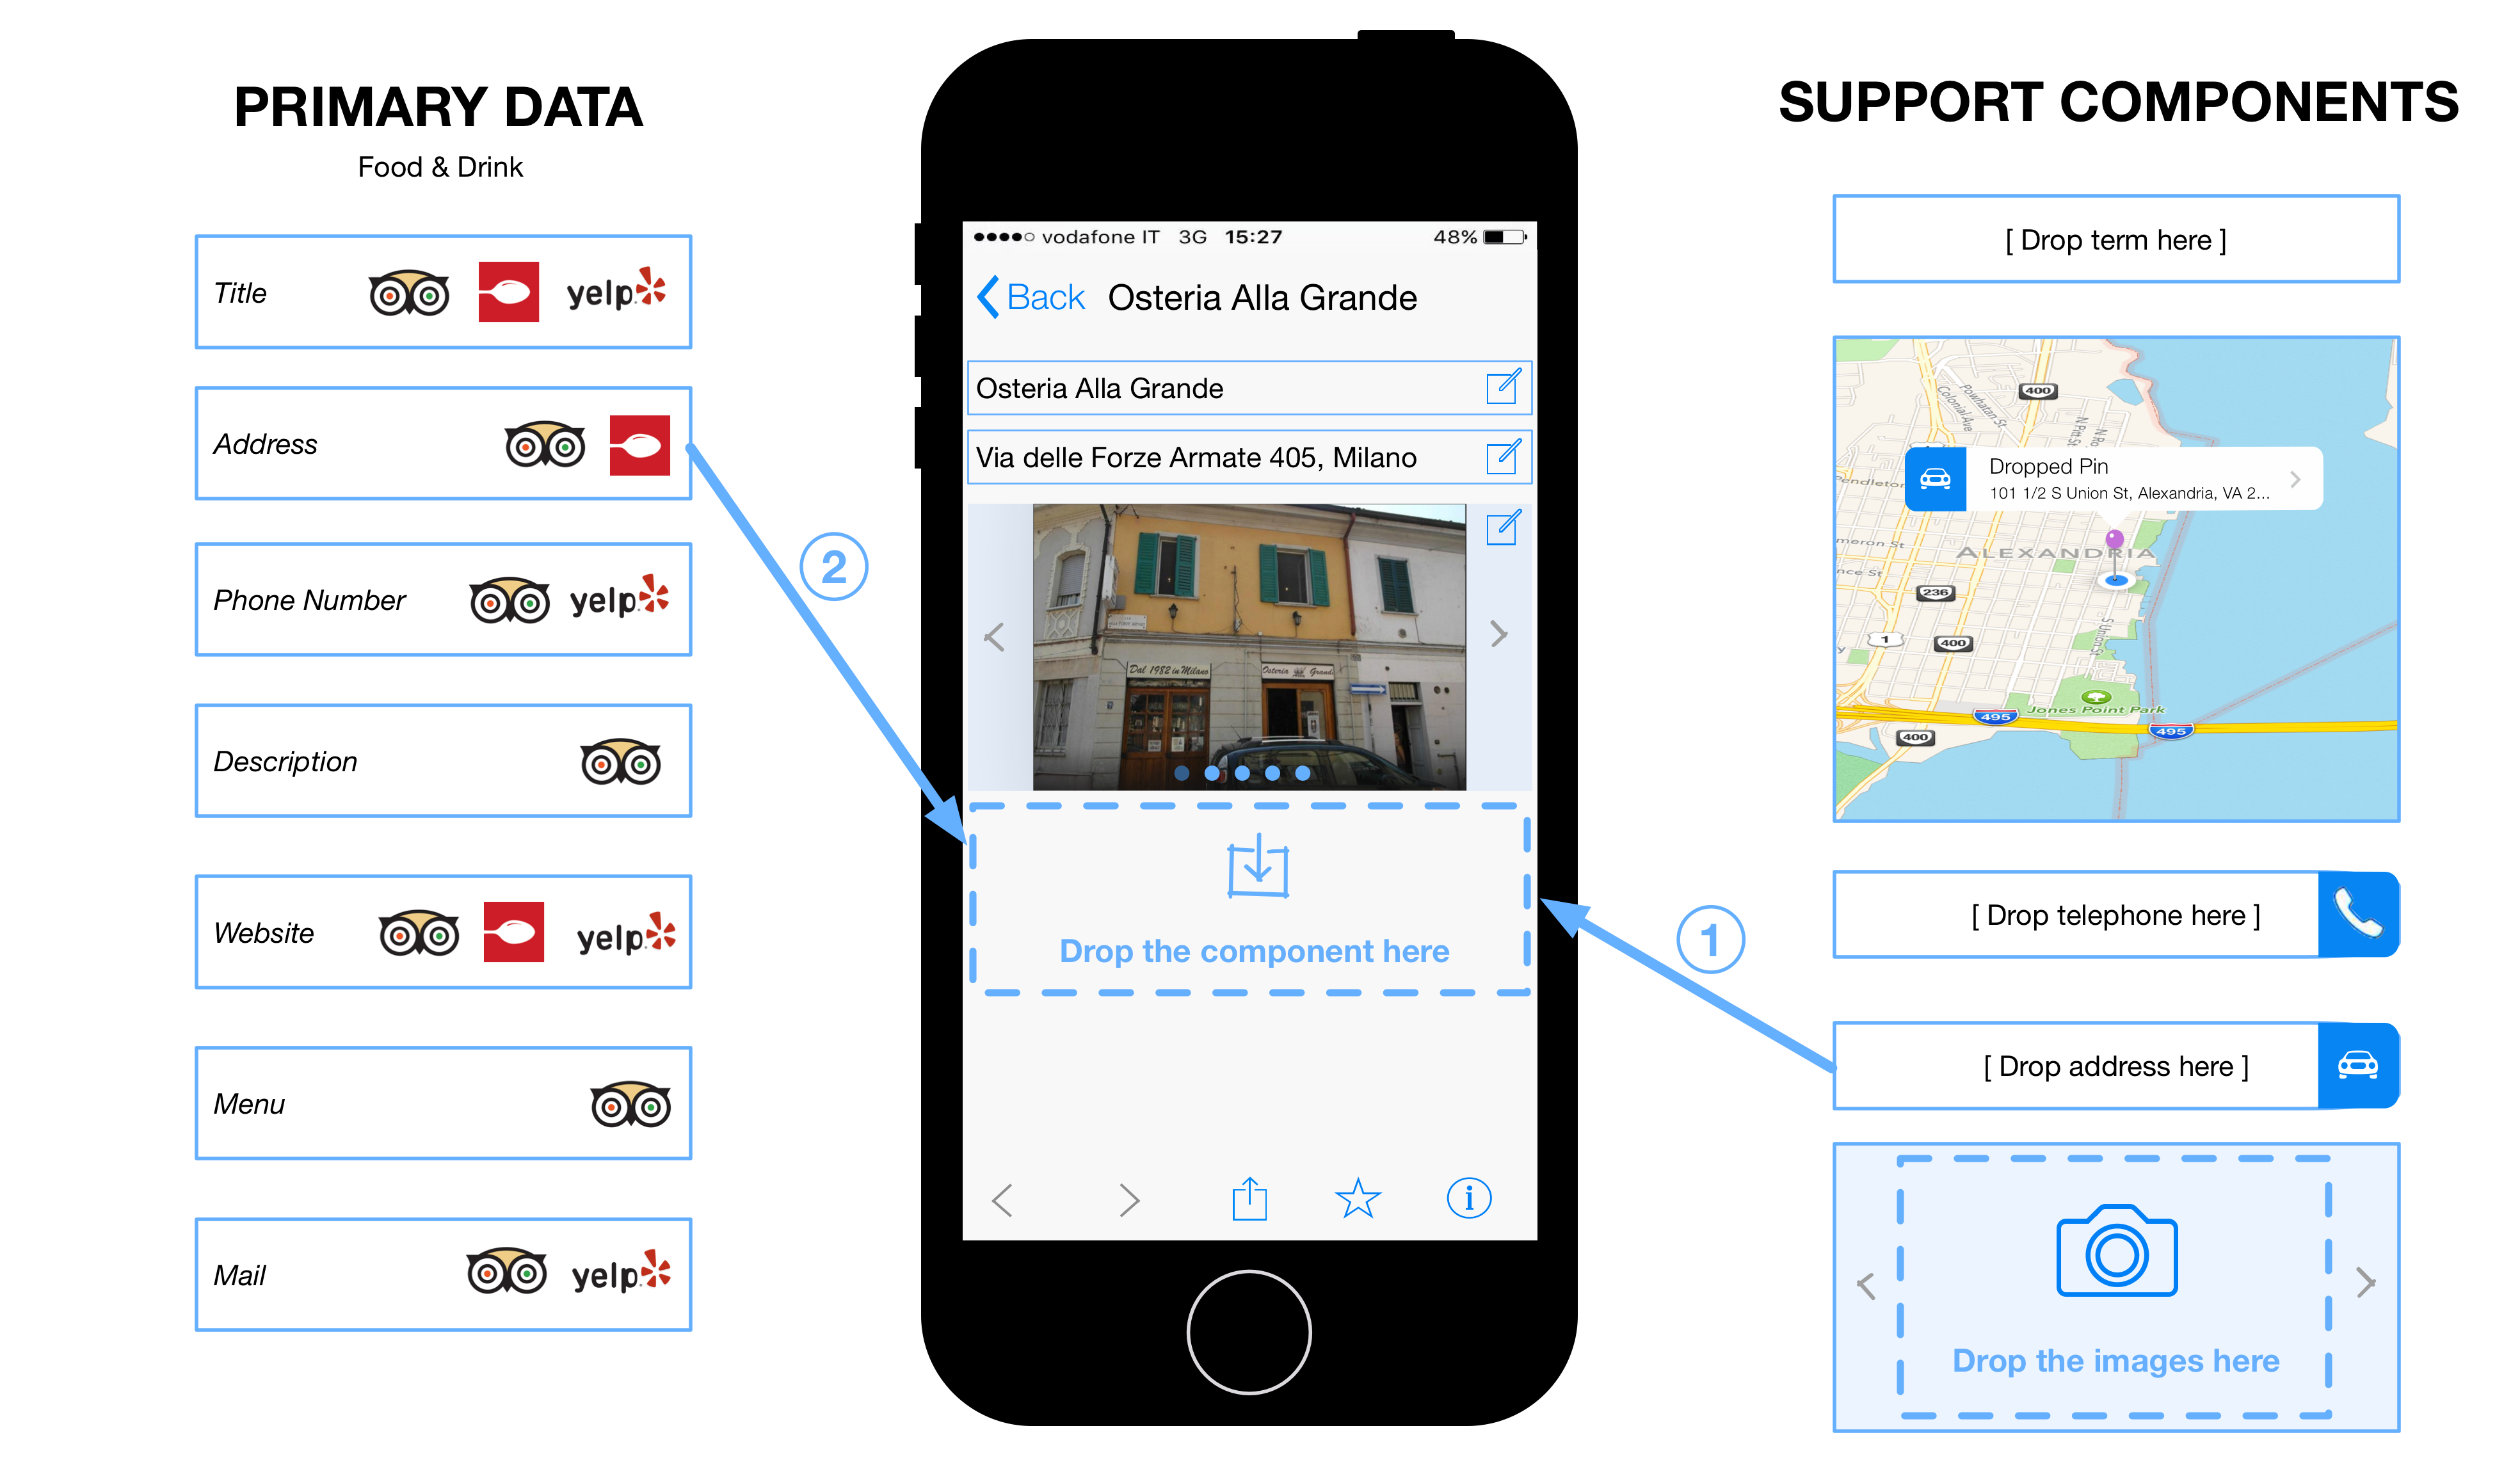
\includegraphics[width=\textwidth]{3-metodologia-camus/Immagini/visual-mapping-nuovo.png}
	\caption{Web App di Visual Mapping}\label{fig:visual-mapping}
\end{figure}

Un altro aspetto fondamentale del sistema è legato all'utilizzo dei mashup per costruire le view dell'applicazione mobile e per associare a ogni singolo elemento delle viste il termine che caratterizza i dati da richiedere al server. Questo compito viene svolto dall'\emph{esperto di settore} per mezzo della web app di Visual Mapping (Figura \ref{fig:visual-mapping}), la quale genera uno schema che definisce come e quali informazioni vengono mostrate all'utente.

\upe stato scelto di adottare due tipologie di schemi fondamentali, uno per la lista dei risultati (UNION) e uno per i dettagli dell'elemento selezionato (MERGE), perché fondamentalmente sono queste due le pagine dell'applicazione che necessitano di istanziare con i dati gli elementi visuali dei template.
Gli schemi generati possono essere ulteriormente differenziati per due motivi principali:

\begin{enumerate}
	\item
	Il primo di essi è la tipologia dei dati, che nel nostro caso viene differenziata usando il parametro dell'\emph{Interest Topic}.
	Per esempio se viene selezionato \virgolette{Food and Drink} può essere necessario visualizzare dati diversi rispetto a \virgolette{Museum}. Anche se ci sono attributi in comune, come \emph{Titolo}, \emph{Indirizzo}, \emph{Numero di telefono}, ci possono essere parametri peculiari, come il tipo di cucina per il primo caso o il tipo di museo per il secondo caso. Questi dati possono essere visualizzati quindi in maniera differente e si è scelto, oltre a una differenziazione a livello di termini, anche di lasciare libertà di scelta per quanto riguarda il design del mashup. 
	\item
	Il secondo aspetto è la possibilità di differenziare i dati da mostrare a livello di utente, dato che non a tutti possono interessare le stesse informazioni oppure può essere preferibile mostrare i dati e le view in maniera differente in stili grafici e componenti. Infatti, una volta generato, lo schema dei mashup viene associato allo specifico utente, in modo da essere disponibile su richiesta della mobile app dopo che è stato effettuato l'accesso.
	Nella web app l'esperto seleziona l'utente per il quale deve generare l'applicazione e, in aggiunta alle modifiche al CDT evidenziate nella Sezione \ref{sec:cdt-su-misura}, carica gli schemi predefiniti che verranno utilizzati come base per lo schema personalizzato per l'utente. In questo modo ogni utente dell'applicazione può avere i propri mashup personalizzati.
	Oltre alla definizione dei termini nei mashup, è possibile aggiungere le proprietà stilistiche relative al singolo schema, se diverse da quelle definite globalmente.
\end{enumerate}

\begin{figure}[ht]
	\centering
	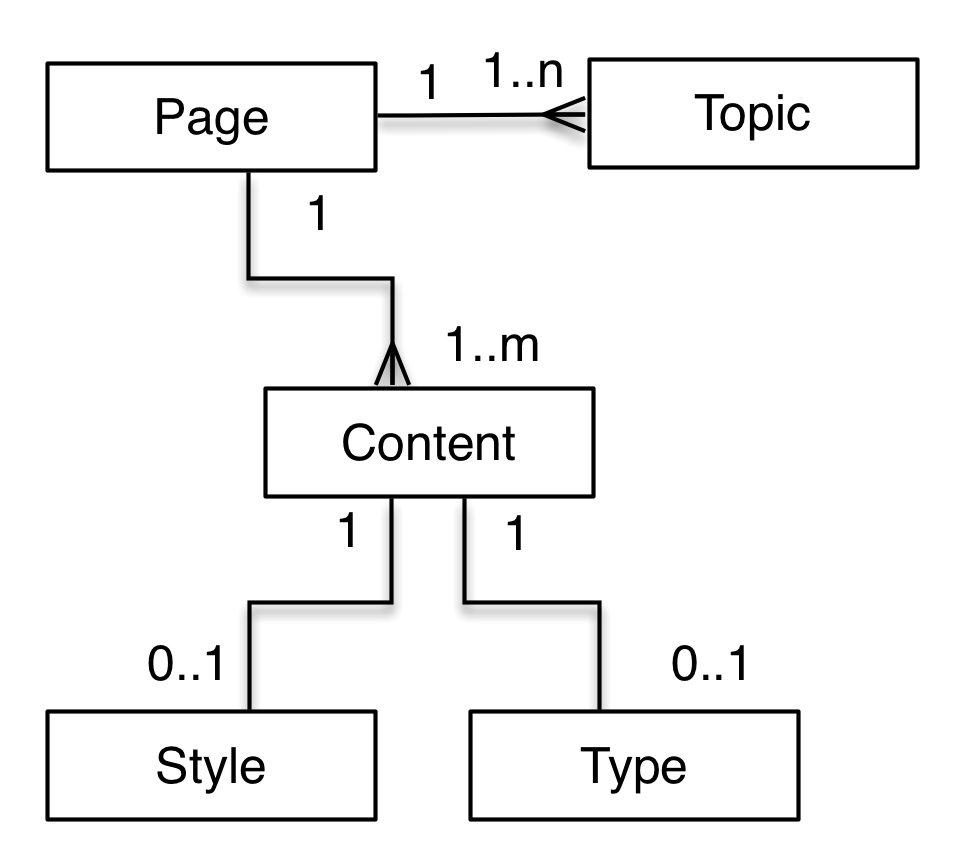
\includegraphics[width=0.4\textwidth]{3-metodologia-camus/Immagini/view-schema.png}
	\caption{Schema delle views}\label{fig:view-schema}
\end{figure}

Lo schema delle view che è stato adottato è raffigurato nella Figura \ref{fig:view-schema}. A ogni pagina definita vengono associati uno o più valori di \virgolette{Interest Topic}, perché può essere che uno schema venga utilizzato in più ambiti. Ogni pagina può avere più di un contenuto al quale è associato opzionalmente uno stile e la tipologia del contenuto, che servirà all'app per renderizzare il componente associato. Per esempio se il designer desidera mostrare il titolo nei dettagli con una dimensione maggiore di quella di default e con un colore rosso, può impostare questi parametri nel campo \virgolette{Styles}. Nella fase di elaborazione dinamica delle view sarà l'applicazione ad applicare questo stile se presente, sostituendo quello di default. Per quanto riguarda la tipologia del dato titolo in questo caso è necessario fornire che è di tipo \virgolette{Text}. Per componenti più complessi come una mappa è sufficiente fornire come tipologia \virgolette{Map} e come contenuti i parametri di latitudine e longitudine per ottenere la visualizzazione desiderata.

Per personalizzare uno schema, al \emph{designer} spettano i seguenti passaggi:

\begin{itemize}
	\item \textbf{Associazione dei termini} 
	L'associazione dei termini agli elementi visuali viene effettuata mediante \emph{drag} \& \emph{drop}. I singoli termini sono collegati allo specifico elemento della view. 
	I termini possono essere acquisiti da una repository mantenuta sul server o da una \emph{knowledge base}\footnote{Schema.org: \url{http://schema.org/}}, che permette di associare un significato semantico a ogni termine in modo da agevolare l'interoperabilità dei dati. Il designer può scegliere se utilizzarli tutti o solo una parte nella creazione dello schema, in modo che a runtime l'applicazione possa richiedere solamente i dati necessari alla popolazione della view.
	Nella Figura \ref{fig:visual-mapping} viene mostrata la sequenza di operazioni che deve compiere il designer e che vengono elencate di seguito:
	\begin{enumerate}
		\item
		Selezione dell'elemento visuale da inserire (es.: text field, mappa, galleria foto, ecc.) nella schermata del telefono e modifica dello stile a seconda delle opzioni disponibili
		\item
		Associazione del termine tra l'elenco di tutti quelli disponibili
	\end{enumerate}
	Per esempio, per mostrare il titolo di un'istanza, l'esperto deve selezionare l'elemento che permette di mostrare del testo, trascinarlo all'interno della schermata virtuale e associarvi il campo titolo dai termini sulla sinistra della web app. A questo punto è possibile modificare alcuni elementi di stile tramite CSS che, definiti sullo schema, sovrascrivono eventuali stili presenti in quello predefinito.
	%allungare questa parte
	\item \textbf{Associazione dei servizi di supporto}
	Come spiegato nella Sezione \ref{sec:ecosistema-servizi}, i servizi di supporto hanno la funzione di arricchire le informazioni che sono fornite dai servizi primari. La loro integrazione nei mashup può essere fatta principalmente in due modi:
	\begin{enumerate}
		\item
		La prima possibilità è di associare a un termine una app già installata sul device. Si consideri il caso d'uso del turismo e un servizio di ristoranti che restituisce un numero di telefono: questo dato può essere collegato al dialer di default per effettuare direttamente una chiamata o all'app di gestione degli SMS. Oppure l'indirizzo email può essere associato alla funzione \virgolette{Crea Email} dell'app predefinita di gestione della posta elettronica. Un altro esempio può essere quello di associare il browser di sistema al sito ufficiale o alle pagine Facebook del ristorante
		\item
		La seconda possibilità riguarda invece l'utilizzo di un modulo che mostri direttamente i risultati dei servizi di supporto all'interno dell'app. In questo modo è possibile mostrare nuovi dati relativi a un singolo elemento proveniente dai servizi primari. \upe possibile per esempio associare una mappa per visualizzare una posizione geografica oppure una segnalazione che indica la distanza o i tempi di percorrenza, oppure, citando sempre l'esempio dei locali, i mezzi pubblici, car sharing o taxi che si possono utilizzare per raggiungere il ristorante
	\end{enumerate}
\end{itemize}